% ------------------------------------------------------------
% LaTeX Template für die DHBW zum Schnellstart!
% Original: https://github.wdf.sap.corp/vtgermany/LaTeX-Template-DHBW
% ------------------------------------------------------------
% ---- Präambel mit Angaben zum Dokument
\input{Inhalt/00_Latex/praeambel}

% ---- Elektronische Version oder Gedruckte Version?
% ---- Unterschied: Die elektronische Version enthält keinen Platzhalter für die Unterschrift
\usepackage{ifthen}
\newboolean{e-Abgabe}
\setboolean{e-Abgabe}{false}    % false=gedruckte Fassung

% ---- Persönlichen Daten:
\newcommand{\titel}{Erkennung fahrradfreundlicher, städtischer Wege mithilfe von Computer Vision über Luftaufnahmen}
\newcommand{\titelheader}{Studienarbeit}
\newcommand{\arbeit}{Studienarbeit}
\newcommand{\studiengang}{Informatik}
\newcommand{\studienjahr}{2022}
\newcommand{\autor}{Dominik Ochs und Franziska Ommer}
\newcommand{\autorReverse}{Ochs, Dominik; Ommer, Franziska}
\newcommand{\verfassungsort}{Karlsruhe}
\newcommand{\matrikelnr}{2847475; 0000000}
\newcommand{\kurs}{TINF20B2}
\newcommand{\bearbeitungsmonat}{August 2022}
\newcommand{\abgabe}{16. April 2023}
\newcommand{\bearbeitungszeitraum}{01.10.2022 - 16.04.2023}
\newcommand{\firmaName}{SAP SE}
\newcommand{\firmaStrasse}{Dietmar-Hopp-Allee 16}
\newcommand{\firmaPlz}{69190 Walldorf, Deutschland}
\newcommand{\betreuerFirma}{Christoph Eckert}
\newcommand{\betreuerDhbw}{Prof. Dr.-Ing. Markus Reischl}

\input{Inhalt/00_Latex/kopfundFusszeile}

% ---- Hilfreiches
\newcommand{\zB}{z.\,B. }   % "z.B." mit kleinem Leeraum dazwischen (ohne wäre nicht korrekt)
\newcommand{\dash}{d.\,h. }

\newcommand{\code}[1]{\texttt{#1}} % Ist einfacher zu schreiben als ständig \texttt und erlaubt
                                   % Änderungen im Nachhinein, wenn man z.B. Inline-Code anders stylen möchte.

% ---- Silbentrennung (falls LaTeX defaults falsch / nicht gewünscht sind)
\hyphenation{HANA}         % anstatt HA-NA
\hyphenation{Graph-Script} % anstatt GraphS-cript
\hyphenation{Performance-tests}

% ---- Watermark/Wasserzeichen
%\input{Inhalt/00_Latex/watermark} % Auskommentieren wenn nicht erwünscht
%\watermark{gray}{\textbf{DRAFT}}     % Auskommentieren wenn nicht erwünscht. Nimmt optional die opacity/Deckraft z.B. \watermark[0.1]{green}{text} für 10% Deckkraft
%\SetWatermarkSize{8} % Optional. Standard ist 5.8. 

% ---- Beginn des Dokuments
\begin{document}
\setlength{\parindent}{0pt}              % Keine Paragraphen Einrückung.
                                         % Dafür haben wir den Abstand zwischen den Paragraphen.
\setcounter{secnumdepth}{2}              % Nummerierungstiefe fürs Inhaltsverzeichnis
\setcounter{tocdepth}{1}                 % Tiefe des Inhaltsverzeichnisses. Ggf. so anpassen,
                                         % dass das Verzeichnis auf eine Seite passt.
%\sffamily                                % Serifenlose Schrift verwenden.

% ---- Vorspann
% ------ Titelseite
\singlespacing
\include{Inhalt/01_Standard/titelseite}  % Titelseite
\newcounter{savepage}
\pagenumbering{Roman}                    % Römische Seitenzahlen
\onehalfspacing

% ------ Erklärung, Sperrvermerk, Abstact
%\include{Inhalt/01_Standard/sperrvermerk}
\include{Inhalt/01_Standard/erklaerung}
\renewcommand{\abstractname}{Abstract} % Veränderter Name für das Abstract
\begin{abstract}
\begin{addmargin}[1.5cm]{1.5cm}        % Erhöhte Ränder, für Abstract Look
\thispagestyle{plain}                  % Seitenzahl auf der Abstract Seite

\begin{center}
\small\textit{- English -}             % Angabe der Sprache für das Abstract
\end{center}

\vspace{0.25cm}


This thesis develops an efficient algorithm for calculating the similarity of two material flow graphs based on the number of common node labels. Material flow graphs are  node-labelled \acp{DAG} with many nodes of outdegree one, which share a common sub-\ac{DAG} whenever they share a node with a common label. \\
It was previously found that comparing two material flow graphs by simply counting their common node labels is inefficient. Rather, this process can be siginificantly sped up by making use of the sharing sub-\ac{DAG} property by, first, reducing the graph to only sink and fork nodes (where fork nodes are nodes with outdegree greater 1), and then comparing the reduced graphs. This allowed for a speed-up of  factor 10 for average problems, whereas the comparison of especially large material flow graphs with very few fork nodes and sinks could be sped up by factor 83 to 168. 


\end{addmargin}
\end{abstract}
\renewcommand{\abstractname}{Abstract} % Veränderter Name für das Abstract
\begin{abstract}
\begin{addmargin}[1.5cm]{1.5cm}        % Erhöhte Ränder, für Abstract Look
\thispagestyle{plain}                  % Seitenzahl auf der Abstract Seite

\begin{center}
\small\textit{- Deutsch -}             % Angabe der Sprache für das Abstract
\end{center}

\vspace{0.25cm}

Diese Arbeit vergleicht einige U-Net-basierte Architekturen und unterschiedliche
Pre-Training-, Fine-Tuning- und Augmentierungs-Methoden zum Erkennen 
und semantisch Segmentieren von städtischen Radwegen aus Luftbildern. 
Dafür werden mehrere Datensätze erstellt und mittels eines eigens entwickelten Algorithmus 
und OpenStreetMap-(OSM)-Daten automatisch annotiert. Um die Ergebnisse zu bewerten, 
wird eine gepufferte Form der \textit{\acf{IoU}}, genannt \textit{\acf{BIoU}}, 
welche eine rasterisierte Version des \textit{Quality}-Maßes darstellt, entwickelt. \hspace{2mm} \\
Die Ergebnisse zeigen mittelmäßigen Erfolg beim Erkennen von Fahrradwegen, insbesondere dann, 
wenn Städte mit abweichender Infrastruktur, die nicht während des Trainings verwendet wurden, getestet werden. 
Der hier verwendete Trainingsdatensatz enthält nur sehr ähnliche Städte und ist teilweise falsch annotiert, 
also können bessere Annotationen, zum Beispiel durch Menschen erstellt,
mit einem Datensatz mit einer größeren Vielfalt an städtischer Infrastruktur 
potentiell bessere Ergebnisse erzielen. Außerdem liefert semantische Segmentierung mehr Information 
als für die Aufgabe notwendig ist, was unnötige Komplexität und schwer zu lernende Details hinzufügt, 
weswegen alternative Herangehensweisen, wie das direkte Extrahieren 
eines Graphens der Radwege im Deep-Learning-Netz selbst, bessere Ergebnisse liefern könnten. 
Hierfür können die OSM-Graphen direkt als Annotation genutzt werden. 
Um die so erhaltenen Graphen mit den Ergebnissen dieser Arbeit zu vergleichen, können 
sie zurück auf die Bilder projiziert werden.
Die unterschiedlichen Architekturen und Trainingsmethoden zeigen keine konsequenten 
Verbesserungen der Performanz und werden als nicht signifikant erachtet. 

\end{addmargin}
\end{abstract}

% ------ Inhaltsverzeichnis
\singlespacing
\tableofcontents

% ------ Verzeichnisse
\renewcommand*{\chapterpagestyle}{plain}
\pagestyle{plain}
\chapter*{Abkürzungsverzeichnis}
\addcontentsline{toc}{chapter}{Abkürzungsverzeichnis} % Hinzufügen zum Inhaltsverzeichnis 

\begin{acronym}[WYSISWG] % längstes Kürzel wird verw. für den Abstand zw. Kürzel u. Text

	% Alphabetisch selbst sortieren - nicht verwendete Kürzel rausnehmen!
	% \acrodefplural{ISBN}[ISBNs]{Internationale Standardbuchnummern}

	\acro{BCE}{Binary Cross Entropy}
	\acro{DC} {Distribution Center}
	\acro{DFS} {Depth-First Search}
	\acro{GSD} {Ground Sampling Distance}
	\acro{IoU} {Intersection over Union}
	\acro{LocMat} {Location Material}
	\acrodefplural{LocMat}[LocMats]{Location Materials}
	\acro{ML}{Machine Learning}
	\acro{ProdDeco}{Product Decomposition}
    \acro{SCP}{Supply Chain Planning}
    \acro{SNP}{Supply Network Planning}
	\acro{SOP}{Sales and Operations Planning}

\end{acronym}

\listoffigures                          % Erzeugen des Abbildungsverzeichnisses 
\listoftables                           % Erzeugen des Tabellenverzeichnisses
\renewcommand{\lstlistlistingname}{Quellcodeverzeichnis}
\lstlistoflistings                      % Erzeugen des Listenverzeichnisses
\setcounter{savepage}{\value{page}}


% ---- Inhalt der Arbeit
\cleardoublepage
\pagenumbering{arabic}                  % Arabische Seitenzahlen für den Hauptteil
\setlength{\parskip}{0.5\baselineskip}  % Abstand zwischen Absätzen
\rmfamily
\renewcommand*{\chapterpagestyle}{scrheadings}
\pagestyle{scrheadings}
\onehalfspacing

\chapter{Motivation}

Im Folgenden wird die Motivation für diese Arbeit, sowie die Relevanz dieser Arbeit in dem Kontext des \textit{\ac{SCP}} dargelegt. Dafür erfolgt zunächst eine kurze Einführung in \ac{SCP} bei SAP und in konkret eine Methode, die angewandt wird, um Rechenzeit zu reduzieren. Daraufhin wird ein Problem bei diesem Verfahren vorgestellt und schließlich die Ziele und das geplante Vorgehen für diese Arbeit diskutiert.

\section{SAP Supply Chain Optimizer} \label{sec:sap_scp}

Das \textit{\ac{SCP}} stellt für viele Unternehmen in einer globalisierten, digitalisierenden Welt mit sich immer schneller verändernden Märkten eine zunehmende Herausforderung dar.n Optimierungslauf wird von den Kunden zumeist  einmal täglich durchgeführt.

\section{Product Decomposition und Similarity} \label{sec:proddeco}

Für besonders große Szenarien kann es wünschenswert oder sogar nötig werden die Komplexität des Szenarios zu reduzieren, um mit geringerem Ressourcenaufwand in Form von Laufzeit und Speicher eine optimierte Lösung   nach \autoref{sec:sap_scp} zu erhalten. Dies kann zum Beispiel mit der \textit{\ac{ProdDeco}} bewerkstelligt werden \cite{.20220812}. Hierfür wird die gesamte Supply Chain in jeweils kleinere \textit{Subprobleme} aufgeteilt. Diese stellen Gruppen aus Produkten dar, die möglichst wenig Berührungspunkte mit anderen Subproblemproduktgruppen haben. Die Subprobleme werden dann individuell und unabhängig voneinander optimiert~\cite[S.~31--33]{Sandner.01.09.1998}.   

In \autoref{fig:sim_alg} ist die Synthese der Subprobleme mithilfe der Similarity illustriert. Dieser Vorgang wiederholt sich bis alle Submodelle zu Subproblemen zugeordnet worden sind (6). \\ %macht zeilenumbruch
Wenn $n$ die Anzahl an atomaren Submodellen ist, folgt direkt aus dem Algorithmus per Gaußscher Summenformel
\begin{align}
\label{eq:num_comp} \#S := \sum_{i=0}^{n} i = \frac{n(n+1)}{2} \in O(n^2)
\end{align}
für die Anzahl der paarweisen Vergleiche und damit die Anzahl der Similarity-Berechnungen $\#S$. \\
Für die Zeitkomplexität der Subproblemsynthese $t_{sub}$ gilt also \autoref{eq:t_sim}, wobei $m$ die durchschnittliche Größe - also die durchschnittliche Anzahl der Elemente - der Submodelle beschreibt.
\begin{align}
	\label{eq:t_sim} t_{sub}(n, m) \in O(\#S \cdot t_{sim}(m)) = O(n^2 \cdot t_{sim}(m)) 
\end{align}

\begin{figure}
	\centering
	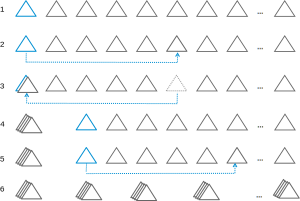
\includegraphics[width=0.80\textwidth]{Bilder/similarity_algorithm.pdf} 
	\caption{Abstrakter Synthesealgorithmus der Subprobleme unter Nutzung der Ähnlichkeit der Submodelle. \\ (In Anlehnung an \cite{Kniasew.21.02.2022}.)}
	\label{fig:sim_alg}
\end{figure} 

\section{Problemszenario} \label{sec:problem}

Als Übergangslösung wurde der Algorithmus für das kritische Szenario so angepasst, dass eine Menge Informationen außer acht gelassen wurden, um auf Kosten der Lösungsqualität eine akzeptable Laufzeit von $14 min$ $47 s$\footnote{Zeit von lokalem Testsystem (s. \autoref{sec:perf})} zu erreichen. \\
Die Supply Chain des Ausgangsszenarios hat hierbei insgesamt ca. 1.97 Mio. Elemente und die 18771 erstellten atomaren Submodelle im Mittel jeweils ca. 5100 Elemente \cite{Kniasew.21.02.2022}. 

Das bedeutet nach \autoref{eq:num_comp} bereits $\#S = \frac{18771 \cdot (18771 + 1)} {2} \approx 176'000'000$ Vergleiche die durchgeführt werden müssen. Für den Worst-Case ist  $t_{sim}$ mit $t_{sim}(m) \in O(m \log m)$\footnote{Auf die Unterscheidung zw. $m_{1}$ und $m_{2}$ wird hier aufgrund des $O$-Kalküls und der Verwendung von $m$ als Mittelwert der Elementzahlen verzichtet.} angegeben \cite{Kniasew.21.02.2022}. Für $m=5100$ ergeben sich die asymptotischen Ungleichungen 
\begin{align}
	t_{sim}(m) \preccurlyeq m \log m \approx 62800 \implies \nonumber \\
	\label{eq:conrete_id_obj} t_{sub}(n, m) \preccurlyeq \#S \cdot m \log m \approx 176'000'000 \cdot 62800 \approx 11 \cdot 10^{12}
\end{align}


\section{Zielsetzung, Inhalt und Vorgehensweise}

Es ist ersichtlich, dass Anlass zur Verbesserung der Laufzeit gegeben ist, um 
\begin{enumerate}
\item das kritische Szenario ohne Weglassen von Informationen durchführbar zu machen und
\item die durchschnittlichen Szenarien zu verbessern, um Rechenzeit und damit langfristig Energie zu sparen.  
\end{enumerate}  
Hierfür wird sich vor allem auf $t_{sim}$ und dessen Minimierung fokussiert. Ziel ist es, eine neue Art der Similarity-Berechnung zu finden, die schneller abläuft als die alte, aber dabei noch die genau gleichen Subprobleme erzeugt. 
% Hier wird der theoretische Teil vorgenommen. 

\chapter{Stand der Technik}

\section{Aufgabenkategorien}

Im Bereich der Computer Vision gibt es verschiedene Kategorien von Aufgaben.
Dazu wird nachfolgend ein Überblick über \textit{Klassifizierung}, \textit{Object Detection} und \textit{Image Semantic Segmentation} gegeben.
Eine Visualisierung ist in \autoref{fig:categories} gegeben.
Die aufgeführten Kategorien nehmen in der genannten Reihenfolge in ihrer Komplexität zu.
Es folgt eine Übertragung auf das zu behandelnde Problem der Fahrradwegsegmentierung.

\begin{itemize}
	\item \textit{Klassifizierung:}
	Eine reine Klassifizierung ist die einfachste Lösungskategorie. 
	Es soll lediglich erkannt werden, welche Klasse in einem Bild enthalten ist.
	Die Lokalität des erkannten Objektes wird vernachlässigt, wichtiger ist die Zuordnung zu einer Klasse.
	Dies lässt sich auch entsprechend auf die Erkennung von mehreren Klassen erweitern.
	
	\item \textit{Object Detection:}
	Eine Erweiterung der Klassifizierung um die Lokalität des erkannten Objektes wird \textit{Image Localization} genannt.
	Für mehrere Objekte wird der Begriff Object Detection verwendet.
	Die Darstellung erkannter Objekte wird über Bounding Boxes realisiert, welche die Objekte jeweils umschließen.

	\item \textit{Image Semantic Segmentation:}
	Die bei der Object Detection verwendeten Bounding Boxes geben keine Rückschlüsse auf die konkrete Form der Klasse.
	Je nach Lage des Objektes kann nur ein Bruchteil der Bounding Box von der erkannten Klasse gefüllt sein.
	Abhilfe schafft die Verwendung einer pixelweisen Maske anstelle einer Bounding Box, das Objekt kann von seiner Umgebung abgegrenzt werden.
	Zusätzlich kann gefordert werden, dass einzelne Instanzen verschiedener Objekte unterschieden werden sollen.
	Diese Forderung wird dann \textit{Instance Segmentation} genannt \cite{Sharma.21.08.2019}.
\end{itemize}

\begin{figure}
	\centering
	\includegraphics[width=0.8\textwidth]{Bilder/categories.png} 
	\caption{Verschiedene Aufgabenkategorien \cite{.10.11.2022}}
	\label{fig:categories}
\end{figure} 

Für die Erkennung von Radwegen wird Image Semantic Segmentation verwendet, da für jeden einzelnen Pixel bestimmt werden soll, ob dieser Bestandteil eines Radweges ist.
Eine einfache Klassifizierung oder Object Detection ist nicht ausreichend, eine Instantiierung verschiedener Radwege übersteigt die gewünschte Anforderung nach dem reinen Erkennen von Wegen.
Aus den gewonnenen Kategorien der einzelnen Pixel lassen sich Masken zeichnen, denen dann die konkreten Verläufe entnommen werden können.

\section{Aktivierungsfunktionen}

Im Folgenden wird der Stand der Technik für Aktivierungsfunktionen in \ac{ML}-Modellen dargelegt,
hierzu werden einige Funktionen kurz vorgestellt und deren Vor- und Nachteile bewertet. 
Die besprochenen Funktionen sind dargestellt in \autoref{fig:activation}.

\subsection{Sigmoid}

Die \textit{Sigmoid}-Funktion bildet die Eingabe auf einen Wert im Intervall $(0;1)$ ab und wird durch \autoref{eq:sigmoid} beschrieben.
Der Vorteil hier ist, dass Aktivierungen nie groß werden können, wodurch einzelne Neuronen nicht den Gradienten dominieren können und 
eine fortlaufende Normalisierung durchgeführt wird. Die Probleme hingegen sind, dass die Funktion eher aufwendig zu berechnen ist 
und dass die Ableitung deutlich flacher verläuft. Hierdurch kann es zum \textit{Vanishing-Gradient-Problem} kommen, wobei 
Neuronen in den flacheren Schichten eines neuronalen Netzes kaum noch geupdated werden \cite[S.~191--192]{Goodfellow.2016}. 
\begin{align}
	\label{eq:sigmoid} Sigmoid(z) = \frac{1}{1+e^{-z}}
\end{align} 

\subsection{\acf{ReLU}}

Die \textit{\acf{ReLU}} ist eine Aktivierungsfunktion, welche durch \autoref{eq:relu} ausgedrückt wird. 
\ac{ReLU} ist inzwischen der de-facto Standard von Aktivierungsfunktionen in den verborgenen Schichten eines Deep-Learning-Modells.
Dies liegt vor allem daran, dass das Vanishing-Gradient-Problem adressiert wird. Allerdings hat \ac{ReLU} das Problem, 
dass Neuronen auf $0$ gesetzt werden, wodurch sie kein Gradienten-Update mehr erhalten und dauerhaft genullt bleiben 
und somit nichts mehr zum Netzwerk beitragen - die Neuronen sterben. Das Problem wird \textit{Dying-\ac{ReLU}-Problem} genannt \cite[S.~189--191]{Goodfellow.2016}. 

\begin{align}
	\label{eq:relu} ReLU(z) = \begin{cases} 
		z & z > 0 \\
		0 & z \leq 0 
	\end{cases}
\end{align} 

\ac{ReLU} erzielt eine höhere Inferenz- und Trainingsgeschwindigkeit bei gleicher oder besserer Performanz, 
als Sigmoid. Dies liegt zum einen an der Verbesserung des Vanishing-Gradient-Problems und zum anderen an der 
simpleren und damit leichter zu berechnenden Funktion \cite[S.~226]{Goodfellow.2016}.

\subsection{\acf{ELU}}

Die \textit{\acf{ELU}} ist eine Aktivierungsfunktion, die das Dying-\ac{ReLU}-Problem adressieren soll. 
Ausgedrückt wird die Funktion durch \autoref{eq:elu}. Die negative Komponente lässt zu, dass Neuronen nicht 
von einem Satz auf $0$ zurückkommen können, und weiterhin etwas zur Zielfunktion beitragen können. Außerdem ist die mittlere 
Aktivierung näher an $0$ als bei \ac{ReLU}, was zur Folge hat, dass das Training schneller konvergiert \cite{Clevert.23112015}.

\begin{align}
	\label{eq:elu} ELU(z) = \begin{cases} 
		z & z > 0 \\
		\alpha \cdot (e^z - 1) & z \leq 0 
	\end{cases}
\end{align}

Sowohl \ac{ReLU} als auch \ac{ELU} haben das Problem, dass Aktivierungen beliebig groß werden können, 
wodurch einige wenige Neuronen den Gradienten dominieren können, was zu langsamen Training und suboptimaler Performanz führen kann - das \textit{Exploding-Gradient-Problem}. 
\begin{figure}
	\centering
	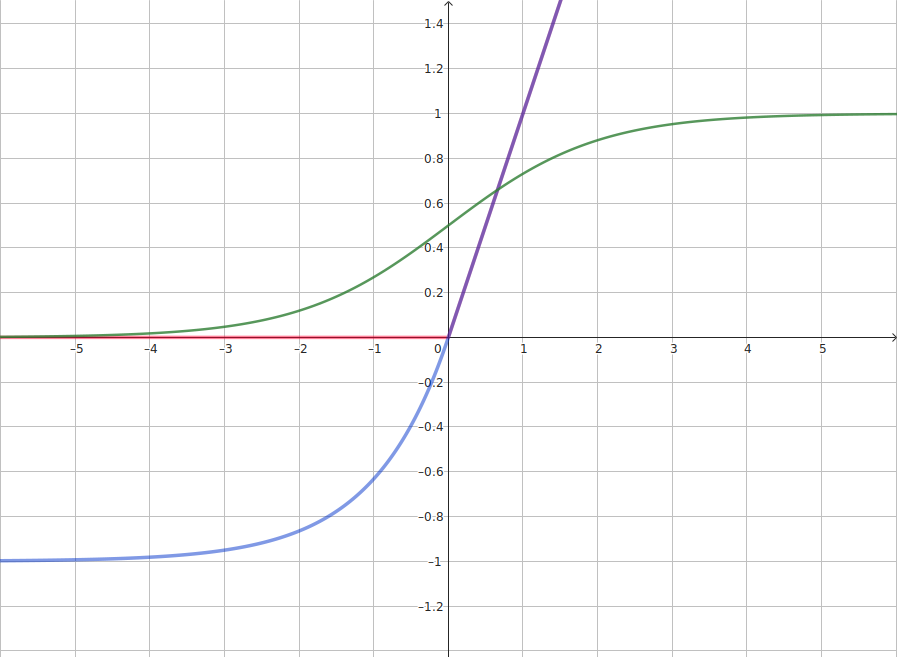
\includegraphics[width=0.8\textwidth]{Bilder/activation-geogebra-export.pdf} 
	\caption{Verschiedene Aktivierungsfunktionen. Grün: Sigmoid. Rot: \ac{ReLU}. Blau: \ac{ELU} mit $\alpha = 1$.}
	\label{fig:activation}
\end{figure} 


\section{Ähnlichkeitsmaße}

Im Folgenden sollen Ähnlichkeitsmaße zwischen Mengen, insbesondere 
solche, die als Kostenfunktion bzw. Bewertungsmetrik für einen binären 
Klassifikator verwendet werden können, untersucht werden. Hierzu wird zunächst Cross-Entropy betrachtet,
gefolgt von dem Dice- bzw. F-Maß. Weiter werden \ac{IoU} und das darauf aufbauende Quality-Maß betrachtet.

\subsection{\acf{BCE}}

Die \textit{Cross-Entropy} (bzw. dt. \textit{Kreuzentropie}) ist ein Maß des Unterschieds zweier
Wahrscheinlichkeitsdistributionen. Im Spezialfall einer binären Wahrscheinlichkeitsvariable 
kann die Cross-Entropy zur \textit{\acf{BCE}} spezialisiert werden, um auf ein binäres 
Klassifikationsproblem angewandt zu werden. 
\autoref{eq:bce} zeigt die Kalkulation von \ac{BCE}, wobei $p \in [0;1]$ die Prediction 
eines binären Klassifikators und $y \in {0,1}$ der Wert des Labels darstellen.
\begin{align}
	\label{eq:bce} BCE = -[p \cdot \log(y) + (1-p) \cdot \log(1-y) ]
\end{align} 
Um über $n$ Prediction-Label-Paare $(p_i; y_i)$ den \ac{BCE} zu berechnen, wird das arithmetische Mittel nach
\autoref{eq:bce-mean} gebildet \cite[S.~82]{Cybenko.1999}[S.~57--59]{Murphy.2012}.
\begin{align}
	\label{eq:bce-mean} BCE = -\frac{1}{n}\sum_{i = 1}^{n}[p_i \cdot \log(y_i) + (1-p_i) \cdot \log(1-y_i) ]
\end{align}

Im Sinne einer differenzierbaren Kostenfunktion im Kontext von \ac{ML} sind \ac{BCE},
\textit{negative Log-Likelihood} und \textit{Logistic-Regression} synonym \cite[S.~249]{Murphy.2012}. 

Aus \autoref{eq:bce-mean} geht hervor, warum \ac{BCE} gut geeignet für Klassifikationsprobleme ist.
Im Gegensatz zum mittleren absoluten Fehler, bei dem ein Fehler linear eingeht, und zum mittleren quadratischen Fehler,
bei dem ein Fehler quadratisch eingeht, geht ein Fehler bei \ac{BCE} exponentiell ein. 
Ein größerer Fehler wiegt also exponentiell stärker als ein kleinerer Fehler. 
Hierdurch werden die Fehler pro Datenpunkt und Klasse sehr klein, 
wodurch gute Performance und gute Generalisierung bei \ac{ML}-Modellen erreicht werden können. \\

Bei stark ungleichmäßiger Klassenverteilung kann es jedoch dazu kommen, 
dass die unterrepräsentierte Klasse kaum noch geschätzt wird, 
da der Fehler einer falsch geschätzten überrepräsentierten Klasse zu stark bestraft wird.
Dadurch lernt der Algorithmus, die unterrepräsentierte Klasse kaum zu schätzen.
Eine Abhilfe dagegen schafft eine Gewichtung der unterschiedlichen Klassen \cite[S.~4]{Ronneberger.18052015}.

\subsection{Dice- und F-Maß}

Das \textit{Dice-}, oder auch \textit{Sorensen-Dice-}Maß $D$ wurde 1945 bzw. 1948 erstmals vorgestellt und genutzt, um die Ähnlichkeit zweier botanischer Stichproben zu ermitteln. Verallgemeinert auf diskrete Mengen $X$, $Y$ kann deren Ähnlichkeit nach Dice $D$ beschrieben werden durch \autoref{eq:dice-coeff}. Es gilt $D \in [0; 1]$ \cites[S.~33]{Srenson.1948}[S.~297]{Dice.1945}. 
\begin{align}
	\label{eq:dice-coeff} D = \frac{2 \cdot | X \cap Y |}{2 \cdot | X \cap Y | + |Y \setminus X| + |X \setminus Y|} 
	=\frac{2 \cdot | X \cap Y |}{|X| + |Y|}
\end{align} 

Angewandt auf boolesche Mengen und binäre Klassifikatoren ist das Dice-Maß gleich dem $F_1$-Maß, das ein Maß für die Qualität eines statistischen Tests darstellt. Dafür sei $X$ nun die Menge der positiven Elemente und $Y$ die Menge der als positiv eingestuften Elemente. Dann ist die \textit{Genauigkeit} oder auch \textit{Precision} gegeben durch
\begin{align}
	\label{eq:precision} precision = \frac{|X \cap Y|}{|Y|}
\end{align}
der Anteil der richtig eingestuften Elemente an allen positiv eingestuften Elementen und die \textit{Trefferquote} oder auch \textit{Recall} gegeben durch
\begin{align}
	\label{eq:recall} recall = \frac{|X \cap Y|}{|X|}
\end{align}
der Anteil der richtig eingestuften Elemente an allen positiven Elementen. \\
Das F-Maß, bzw. genauer das $F_1$-Maß, ist dann gegeben durch das harmonische Mittel aus Precision und Recall, wobei $tp$ die Anzahl von wahr-positiven, $fp$ die Anzahl von falsch-positiven und $fn$ die Anzahl von falsch-negativen Elementen ist \cite{YutakaSasaki.2007}:
\begin{align}
	\label{eq:f1} F_{1} = \frac{2\cdot precision \cdot recall}{precision + recall} = \frac{2\cdot tp}{2 \cdot tp + fp + fn}
\end{align}
Precision und Recall können mit einem Faktor $\alpha$ unterschiedlich zueinander gewichtet werden, um mit $F_{\alpha}$ unterschiedliche Aspekte zu fokussieren. 

Das Dice-, bzw. $F_{\alpha}$-Maß kann leicht für eine differenzierbare Kostenfunktion genutzt werden mit Dice-Loss $D_{L}(X, Y) = 1 - D(X,Y)$, bzw. $F_{\alpha}$-Loss $F_{\alpha L}(X,Y) = 1 - F_{\alpha}(X,Y)$. 


\subsection{\acf{IoU}}

Die \textit{\acf{IoU}-} bzw. \textit{Jaccard-Ähnlichkeitsmetrik} ist ein weit verbreitetes Maß zur Bestimmung der Ähnlichkeit zwei diskreter Mengen. Hierzu seien $X$ und $Y$ diskrete Mengen. Dann ist die $IoU$ gegeben durch 
\begin{align}
	\label{eq:iou} IoU = \frac{|X\cap Y|}{|X \cup Y|} = \frac{| X \cap Y |}{| X \cap Y | + |Y \setminus X| + |X \setminus Y|}~.
\end{align} 
Für ein binäres Klassifikationsproblem lässt sich die $IoU$ ausdrücken durch 
\begin{align}
	\label{eq:iou-binary} IoU = \frac{tp}{tp + fp + fn}~,
\end{align}
wobei $tp$, $fp$, $fn$ wie in \autoref{eq:f1} \cite{Fletcher.2018}. 

Auffällig ist die Ähnlichkeit zum Dice- bzw. $F_{1}$-Maß. Es ist allerdings anzumerken, dass bei Dice/$F_1$ die $tp$, also die wahr-positiven, stärker gewichtet werden, als bei der \ac{IoU}. Die augenscheinliche Ähnlichkeit lässt sich durch die Beziehungen
\begin{align}
	\label{eq:dice-iou} IoU = \frac{D}{2 - D} \\
	D = \frac{2 \cdot IoU}{1 + IoU}
\end{align}
beschreiben.
Im Gegensatz zur \ac{IoU} wird beim Dice-Maß eine höhere Gewichtung auf die wahr-positiven Elemente 
gelegt.

\subsection{Quality}

Bei der \textit{Quality} handelt es sich um eine gepufferte Form des \ac{IoU},
die toleranter bezüglich der Lokalität der Elemente der verglichenen Mengen, oder konkreter,
der Pixel einer semantischen Segmentierung, ist, 
wobei für dieselbe Eingabe $Quality \geq IoU$; $Quality \in [0;1]$ gilt, abhängig von der Puffergröße. 
Die Quality wird analog zur \ac{IoU} über eine gepufferte Precision - die \textit{Correctness} - 
und über einen gepufferten Recall - die \textit{Completeness} - berechnet. Insbesondere werden einige Elemente, 
die zuvor als $fp$ und $fn$ eingeordnet wurden, hiermit zu $tp$ konvertiert. \\
Die Quality soll einige Probleme der \ac{IoU} beheben, um ein Ähnlichkeitsmaß darzustellen, 
was näher an der praktischen und vom Menschen wahrgenommen Leistung eines \ac{ML}-Modells zur semantischen Segmentierung liegt.
So soll relativiert werden, dass vor allem im Randbereich einer Segmentierung einzelne abweichende Pixel
nicht als falsch anerkannt werden, sodass die Segmentierung im Großen und Ganzen als richtig anerkannt wird \cite{ChristianWiedemann.1998}. 


\section{Architekturkomponenten}

Im Folgenden werden verschiedene Architekturkomponenten diskutiert, die im \ac{ML} allgemein 
bzw. bei semantischer Segmentierung im Speziellen verwendet werden. Hierzu werden zunächst Dropout-Layer 
und Batch-Normalization-Layer begutachtet und dann die U-Net-Architektur zur semantischen Segmentierung vorgestellt. 

\subsection{Dropout}

\textit{Dropout} ist eine ressourcenschonende Regularisierungstechnik für \ac{ML}-Modelle. 
Hierbei werden einzelne Neuronen mit einer Wahrscheinlichkeit von \textit{Rate} $r$ während des Trainings 
deaktiviert, also deren Output auf $0$ gesetzt.\\ 
Da bei der Inferenz Dropout dazu führen kann, 
dass wichtige Features ignoriert werden, ist Dropout während der Inferenz unerwünscht. Ohne Dropout während der 
Inferenz sind allerdings alle Gewichte aktiv, was zu einer höheren Summe der Gewichte während der Inferenz, 
als während des Trainings führt. Deswegen müssen die Gewichte für die Inferenz nach unten skaliert werden. 
Alternativ können während des Trainings alle Gewichte nach oben skaliert werden, die nicht deaktiviert wurden. 
Somit muss für die Inferenz keine Anpassung vorgenommen werden. Nach jedem Trainings-Batch werden die aktivierten 
Neuronen dann um Faktor $\frac{1}{1-r}$ skaliert werden \cites[S.~255--258]{Goodfellow.2016}{NitishSrivastava.2014}.

Es hat sich gezeigt, dass Dropout eine effektivere Regularisierungstechnik zur Minderung von Overfitting ist, 
als andere ressourcenschonende Techniken, wie \textit{Weight-Decay}, \textit{Filter-Norm-Constraints} oder 
\textit{Sparse-Activity-Regularization}, wobei Dropout mit diesen kombiniert werden kann, für noch bessere 
Regularisierung \cites[S.~265]{Goodfellow.2016}.

\subsection{Batch-Normalization}

\textit{Batch-Normalization} normalisiert und standardisiert den Output von Neuronen auf Basis des Mittelwerts 
und der Streuung einer Batch während des Trainings. Für die Inferenz werden Durchschnittswerte 
des Mittelwerts und der Streuung der Batches des Trainingsdatensatzes herangezogen und angewandt. \\
Batch-Normalization führt zu einer schnelleren Konvergenz im Training, 
sodass die Anzahl an benötigten Epochen in manchen Fällen halbiert werden können. Des Weiteren führt 
Batch-Normalization zu einer gewissen Regularisierung, da es die Kostenfunktion zu einem gewissen Grad glättet 
\cites[S.~317--320]{Goodfellow.2016}{Ioffe.11022015}.
Besonders gut funktioniert Batch-Normalization für \acp{CNN} und Netzwerke mit Sigmoid-Aktivierungsfunktion
\cites[S.~425]{Goodfellow.2016}.

\subsection{U-Net}

Die \textit{U-Net-Architektur} beschreibt eine \textit{Fully-Convolutional-Network-Architektur}, die erstmals in Freiburg 2015 vorgestellt wurde 
und herausragende Ergebnisse für verschiedene Benchmarks, insbesondere zur semantischen Segmentierung kleiner Datensätze, liefert. \\
Aus \autoref{fig:u-net-architecture} geht die namensgebende Architektur der U-Net hervor. Die folgenden Besonderheiten 
führen zu der sehr guten Performanz des Netzes bei semantischer Segmentierung \cite{Ronneberger.18052015}:
\begin{itemize}
	\item Das Netz besteht aus einem kontrahierenden Encoder-Teil (linke Hälfte) und einem expandierenden und symmetrisch aufgebauten
	Decoder-Teil (rechte Hälfte). Der Encoder erzeugt feinere \textit{Feature-Maps} mit zunehmender Netztiefe, 
	während der Decoder diese wieder extrapoliert, was zu einer besseren Lokalisierung führt. 
	\item Zwischen den jeweiligen symmetrischen Encoder- bzw. Decoder-Blöcken befinden sich \textit{Skip-Connections}\footnote{\textit{copy and crop} in der Abbildung.}.
	Zusammen mit dem vorherigen Punkt erhöht dies weiter die Lokalisierung und Performanz, da der jeweilige Decoder-Block feinere Features von der \textit{Up-Convolution}\footnote{implementiert als \textit{Transposed Convolutions}.},
	wie auch den größeren Kontext von früheren Blocks mittels Skip-Connection erhält. 
	\item Zur Mitte des Netzes hin erhöht sich die Anzahl der Convolution-Filter und damit die Anzahl der \textit{Channel}, 
	während sich die Dimensionen der einzelnen Feature-Maps durch das \textit{Downsampling} verringert. 
	Hierbei ist anzumerken, dass bei der Implementation kein \textit{Padding} für die Convolutions verwendet wurde,
	wodurch sich die Dimensionen der Feature-Maps nach jeder Convolution verringert. 
	Hieraus folgt ein Zuschneiden für die Skip-Connections. 
\end{itemize}

\begin{figure}
	\centering
	\includegraphics[width=0.8\textwidth]{Bilder/u-net-architecture.png} 
	\caption{Ursprüngliche U-Net-Architektur \cite{Ronneberger.18052015}.}
	\label{fig:u-net-architecture}
\end{figure} 


\section{Vortrainierte \ac{CNN}-Modelle} \label{sec:pretrained-backbones}

Im Folgenden wird eine Auswahl an \ac{CNN}-Modellen vorgestellt, von denen es öffentlich zugängliche,
vortrainierte Instanzen zur freien Verwendung gibt. 
Die Klassifikations-Modelle sind auf dem ImageNet-Datensatz, der über 14 Mio. Bilder 
mit 1000 Klassen enthält, trainiert.    

\subsection{VGG16} \label{sec:pretrained-backbones:vgg16}

\textit{VGG16} ist ein \ac{CNN}, welches 2015 von der \textit{Visual Geometry Group} vorgestellt wurde 
und zu der Zeit bahnbrechende Ergebnisse bei der Bilderklassifizierung lieferte \cite{Simonyan.04092014}. 
Inzwischen ist es ein Standard-Netz, auf welchem viele weitere Architekturen aufbauen,
um verschiedene Verbesserungen zu realisieren. 
Dadurch ist es auch sehr beliebt für Transfer-Learning. 

\autoref{fig:vgg16-architecture} zeigt die Architektur. VGG16 besteht aus fünf Blöcken mit $3x3$-Convolution-Schichten,
gefolgt von drei Fully-Connected-Schichten. Die ersten beiden Convolution-Blöcke haben zwei Convolution-Schichten,
die letzten drei Blöcke dagegen jeweils drei. 
Jeder Convolution-Block wird gefolgt von einer Maxpool-Schicht und jeder bis auf den vorletzeten verdoppelt die Filteranzahl in den Convolution-Schichten,
beginnend bei 64 Filtern im ersten Block bis hin zu 512 Filtern in den letzten beiden Blöcken \cite{Simonyan.04092014}. 

Das gesamte Netz besitzt 138 Mio. Parameter. Werden die drei Fully-Conntected-Schichten am Ende ausgelassen, 
sind es ungefähr 14,7 Mio. Parameter. 

\subsection{ResNet34} \label{sec:pretrained-backbones:resnet}

Damit Modelle mehr und feinere Features lernen können, müssen sie in der Lage sein, sehr komplexe Funktionen darzustellen. 
Das führt dazu, dass tiefere Netze auf dem ImageNet-Datensatz tendenziell bessere Ergebnisse erzeugen, als flachere. 
Hierin lag auch der Erfolg von VGG16 bzw. VGG19. Jedoch führt das einfache Vertiefen von Netzen zu dem Degredation-Problem, wonach 
flachere Netze besser performen, als tiefere, da die tieferen sehr schwer zu trainieren sind. \\
Dieses Problem adressiert \textit{ResNet} erfolgreich, indem \textit{Residual-Blocks} eingeführt werden. 
Hierdurch können mit \textit{ResNet} tiefere Netze erstellt werden als bisher, die trotzdem noch effizient trainiert werden können.
Ein Residual-Block besteht dabei aus zwei Convolutional-Layer mit einer Skip-Connection zwischen Input der ersten Layer und Output 
der zweiten Layer. Durch die Skip-Connections kann bei der Backpropagation der Gradient ungehindert rückwärts laufen, 
um so auch die flachen Layer upzudaten. So kann z.B. \textit{ResNet34} 34 trainierbare Layer haben, 
während zuvor mit VGG nur 16 bzw. 19 effektiv waren \cite{He.10122015}. 

Die Architektur ist dabei sehr simpel. Sie ist zu sehen in \autoref{fig:resnet34-architecture} 
und stellt - im Falle von ResNet34 - im Prinzip 33 Convolutional-Layer mit wiederholtem Downsampling 
und Skip-Connections zw. jeweils zwei Convoltuional-Layern, gefolgt von einer Fully-Connected-Layer dar \cite{He.10122015}.

ResNet34 hat 63,5 Mio. Parameter. 


\subsection{DenseNet121} \label{sec:pretrained-backbones:densenet121}

\textit{DenseNet121} wurde 2018 erstmals vorgeschlagen und wurde designed, um das Vanishing-Gradient-Problem 
zu verbessern, bessere Feature-Übertragung in tiefere Netzschichten zu ermöglichen und das Wiederverwenden von Features 
zu unterstützen, um somit die Anzahl der benötigten Parameter deutlich zu reduzieren, bei gleichbleibender Performanz \cite{Huang.25082016}.

\autoref{fig:densenet121-architecture} zeigt die Architektur. Was aus der Abbildung nicht ersichtlich ist, ist wie die 
Dense-Blöcke aufgebaut sind: Jede angegebene Convolution-Schicht besteht aus einer Batch-Normalization-Schicht mit \ac{ReLU}-Aktivierung,
gefolgt von der angegebenen Convoltuion-Schicht. Außerdem - und hier liegt die große Erweiterung des DenseNet - sind alle 
Convolution-Schichten eines Dense-Blocks mit allen nachfolgenden Convolution-Schichten des Dense-Blocks konkateniert,
anstatt nur mit dem einen Nachfolgenden, wie es zum Beispiel bei VGG16 der Fall ist. 

DenseNet121 enthält circa 7 Mio. Parameter. Ohne die letzte Fully-Connected-Schicht sind es noch circa 6,9 Mio. 
Bei nur halb so vielen Parametern erreicht DenseNet121 leicht bessere Ergebnisse als VGG16 auf dem ImageNet-Datensatz 
(93\% ggü. 92\% Accuracy für ImageNet-Top5) \cite{Huang.25082016}. 


\section{Transfer-Learning mit U-Net}

\textit{Transfer-Learning} beschreibt das Übertragen von trainierten Gewichten eines \ac{ML}-Modells auf ein anderes, 
bestenfalls ähnliches Problem und Modell. Das Modell wird dann via \textit{Fine-Tuning} verfeinert mit dem neuen Datensatz und unterschiedlichen Trainingsmethoden.
Häufig wird dafür ein Teil des Modells eingefroren, sodass sich die eingefrorenen Gewichte nicht verändern können. Dies verhindert, 
dass die bereits vortrainierten Gewichte durch die erste Trainings-Batch zerstört werden. Eine weitere Möglichkeit ist,
mit einer sehr geringen Lernrate das gesamte Modell zu trainieren. Oft werden beide Ansätze auch verbunden.

Der Vorteil von Transfer-Learning liegt darin, dass das Training deutlich kürzer dauert, 
weil direkt mit einer höheren Genauigkeit eingestiegen wird, mit kleineren Datensätze bessere Ergebnisse erzielt werden können
 und auch insgesamt eine höhere Genauigkeit 
am Ende des Trainings erreicht wird, als bei herkömmlichen Training. Diese Effekte sind verstärkt, 
abhängig davon, wie ähnlich der Datensatz des Pre-Trainings und des eigentlichen Trainings sind \cite{Ruder.3212017}. \\
Insbesondere bei Computer-Vision ist Transfer-Learning effektiv, da bei Bildern high-level Features wie Clustering 
ähnlichfarbener Pixel oder Kantenerkennung oftmals sehr ähnlich zwischen unterschiedlichen Datensätzen ausfallen 
und damit schon vorhanden sind \cite{Ruder.3212017}. 

Für Transfer-Learning mit U-Nets gibt es verschiedene Strategien: Backbone-Netze als Encoder, 
partielles Einfrieren verschiedener Netzbereiche und direktes Trainieren mit geringer Learning-Rate.
Der Stand der Wissenschaft diesbezüglich wird im Folgenden vorgestellt. 

\subsection{Training mit Backbones}

Im Kontext von Transfer-Learning bei U-Nets bezeichnet ein \textit{Backbone} ein etabliertes vortrainiertes \ac{CNN}, 
welches, leicht modifiziert, als Encoder für das U-Net verwendet wird. Hierbei wird der Decoder-Teil des U-Net 
symmetrisch dem Encoder nachempfunden und an passenden Stellen Skip-Verbindungen zwischen En- und Decoder eingebaut. \\
Hierdurch kann eine geeignete \ac{CNN}-Architektur für das spezifische Problem ausgewählt werden. Des Weiteren sind diese 
Modelle auf sehr großen Datensätzen, wie \textit{ImageNet}, vortrainiert öffentlich zugänglich. 

Bei der semantischen Segmentierung von medizinischen Lungen-Ultraschall-Bildern, wurden die besten Ergebnisse von einem Dice-Maß-Standpunkt aus, 
mit einem U-Net mit auf ImageNet trainierten \textit{VGG16}-Backbone erzielt. Das Vergleichsnetz, welches zuerst auf dem \textit{Salien Object}
Datensatz vortrainiert wurde, erzielte schlechtere Ergebnisse von dem Dice-Maß her, wobei allerdings das VGG16-U-Net kleine falsch-positive 
Regionen erkannte, die weit Außerhalb der Ground-Truth lagen. Die falsch-positiven beim Vergleichsnetz, lagen direkt an der Ground-Truth, 
dies lässt auf eine sensitivere Kantenerkennung beim VGG16-U-Net schließen, die manchmal aber auch übersensitiv war \cite{Cheng.05.10.2021}. 

Für das Training des VGG16-U-Nets wurde der Encoder-Teil eingefroren und somit nur der Decoder trainiert. 

\subsection{Partielles Einfrieren und Training mit geringer Lernrate}

Im oben beschriebenen Problem zur semantischen Segmentierung wurde das vortrainierte Vergleichsnetz auf zwei Weisen fein-trainiert:
\begin{enumerate}
	\item Ohne Einfrieren mit einer Lernrate von $10^{-5}$
	\item und mit Einfrieren des mittleren Blocks, welcher ungefähr $14\cdot 10^6$ der insgesamt $31 \cdot 10^6$ Parameter enthielt. 
\end{enumerate}
Die 5-fache Kreuzvalidierung ergab sowohl für den besten Lauf, als auch für den durchschnittlichen Lauf, ein besseres Dice-Maß 
für das Training aller Parameter. In keinem der Fälle gab es, anders als beim VGG16-U-Net, segmentierte Regionen ohne Zusammenhang mit der Ground-Truth \cite{Cheng.05.10.2021}. 

In einem weiteren Paper wurde untersucht, welche Layer eines U-Net am besten eingefroren werden sollten, für das Fine-Tuning von medizinischen Bildern - 
zum einen von Lungen-Ultraschall-Bildern und zum anderen von Brust-Röntgen-Aufnahmen. 
Hier wurde wieder mit dem \textit{Salien Objetcs} Datensatz vortrainiert. Dann wurden für beide Anwendungsfälle folgende Tests durchgeführt: 
\begin{enumerate}
	\item Einfrieren der linken Hälfte (Encoder) des Netzes,
	\item Einfrieren der rechten Hälfte (Decoder) des Netzes,
	\item gesamtes Netz, bis auf den ersten Block eingefroren und dann nach jeweils fünf Epochen sukkzessive weitere Blöcke freigeben und
	\item dasselbe allerdings von hinten nach vorne.
\end{enumerate}
Für die Röntgenaufnahmen gab es keine Unterschiede, wobei der Dice-Score hier allerdings auch bei $0.98$ lag. 
Für die Ultraschallbilder lieferte Methode (1) die schlechtesten Ergebnisse (Dice: $0.72$), gefolgt von Methode (2) (Dice: $0.80$) 
und gleichermaßen (3) und (4) (Dice: $0.82$), wobei (3) deutlich schneller konvergierte \cite{Amiri.19.02.2020}.



\section{Aktueller Stand und Benchmarks} % ...der straßen detection

Die aktuellen State-Of-The-Art-Methoden zur Extraktion von Straßen aus Satelliten- und Luftbildern verwenden 
alle Computer-Vision mittels \acp{CNN} und dabei ausschließlich Netze aus der U-Net-Familie - also angepasste, 
erweiterte, abgeänderte U-Nets \cites{C.Henry.2021, Constantin.2018, Kamiya.2018, Yerram.2022}. \\
Dies liegt vor allem daran, dass das U-Net, welches ursprünglich für biomedizinische Bilder entworfen wurde, 
genau die Probleme adressiert, die auch beim Segmentieren von Straßen auf Luftbildern auftreten. 
Wie auch in medizinischen Bildern leiden die Luftbilder-Datensätze häufig unter großer Klassen-Imbalance 
und unter ähnlichen Annotationsfehlern. Außerdem haben viele medizinische Bilder und Luftbildaufnahmen von Straßen 
ähnliche Topologien. Komplexere Architekturen zur semantischen Segmentierung, wie zum Beispiel solche 
für Bodenaufnahmen-Datensätze (vgl. KITTI \cite{Geiger.2013}) erreichen nicht die Performance von U-Nets bei 
Luftbild-Benchmarks \cite{C.Henry.2021}. \\
Weiter wird die Extraktion von Straßen aus Satelliten- bzw. Luftbildern zumeist in zwei Phasen eingeteilt: 
\begin{enumerate}
	\item Das Erstellen einer binären Maske zu den Luftbildern mittels semantischer Segmentierung, 
	welche die Straßen pixelweise induziert. 
	\item Das Extrahieren eines topologischen Graphens, welcher die Straßen-Zentrumslinien beschreibt.   
\end{enumerate}
Schritt (1) wird dabei zumeist von U-Net-Derivaten behandelt, wobei es allerdings auch Vorschläge von Netzen gibt, 
die direkt Schritt (2) ausführen \cite{C.Henry.2021}.
Im Folgenden wird weiter Schritt (1) betrachtet.   

Der Vergleich von unterschiedlichen Netzen, Papern und Ergebnissen zu der Sache ist häufig erschwert, 
da es trotz gleicher Bewertungsmaße wie Dice oder \ac{IoU}, zwei unterschiedliche gängige Kodierungen gibt:
\begin{enumerate}
	\item Das verwendete \ac{CNN} hat je Input-Neuron bzw. -Pixel $p$ genau ein Output-Neuron $o_p$, welches den jeweiligen Input-Pixel $p$
	als Straße identifiziert, genau dann, wenn der Wert des Output-Neuron $o_p$ einen gewissen Grenzwert $l$ überschreitet ($o_p > l$), 
	ansonsten ($o_p \leq l$) gilt der Pixel $p$ \textit{implizit} als Nicht-Straße, bzw. \textit{Hintergrund}. \\
	In diesem Fall stellt ein korrekt als Hintergrund klassifizierter Pixel ein wahr-negatives Ergebnis dar. 
	Wahr-Negative werden von Dice, bzw. \ac{IoU} allerdings nicht berücksichtigt (vgl. \autoref{eq:f1} und \ref{eq:iou-binary}).
	Ein so klassifizierter Pixel ändert also nichts an dem Score. Es werden nur Straßen betrachtet, nicht aber der Hintergrund.    
	\item Das verwendete \ac{CNN} hat je Input-Neuron bzw. -Pixel $p$ \textit{zwei} Output-Neuronen $\mathbf{o_p} = (o_{p_S}, o_{p_H})$, 
	wobei dies eine One-Hot-Kodierung von Punkt (1) darstellt. 
	Ein Hintergrund-Pixel wird nun \textit{explizit} als solcher klassifiziert. 
	Dies ändert allerdings die Berechnungsgrundlage von Dice und \ac{IoU} erheblich, da diese nun (zumeist) als Mittelwert 
	der Scores zu $o_p{_S}$ und $o_p{_H}$ berechnet werden. Hierdurch fließen die zuvor unberücksichtigten wahr-negativen 
	Hintergrundpixel als wahr-postive in den Dice- bzw. \ac{IoU}-Score ein. Die Verzerrung wird noch verstärkt, 
	da eine starke Imbalance zwischen Straßen- und Hintergrundpixel herrscht, wodurch der Dice-/\ac{IoU}-Score bei 
	der One-Hot-Kodierung viel mehr eine Aussage darüber trifft, wie viele Hintergrundpixel, von denen es ja viel mehr gibt,
	richtig klassifiziert wurden. Die so erzielten Dice-/IoU-Werte sind hier rein numerisch deutlich höher. 
\end{enumerate}

\autoref{tab:basline-benchmarks} zeigt Resultate zum Massachusetts- und Deep-Globe-Datensatz von sogenannten \textit{Basline}-Modellen.
Hierbei handelt es sich um verschiedene Architekturen, die allerdings nicht extrem auf den jeweiligen Datensatz optimiert sind,
was die Hyper-Parameter oder manche Architektur-Anpassungen angeht. Ein Beispiel dafür wäre das Ausprobieren von verschiedenen (Kompositions-)Kostenfunktionen. 
Mit den Baseline-Resultaten können diese Modelle zu Vergleichszwecken verwendet werden 
und es bestehen Daten zu mehreren Benchmarks \cite{C.Henry.2021}.

\begin{table}
	\centering
	\begin{tabular}{l|l|l|l|l}
		\multirow{2}{*}{Model} & \multicolumn{2}{c|}{Massachusetts} & \multicolumn{2}{c}{Deep Globe}  \\
		& Dice & IoU & Dice & IoU \\
		\midrule
		DeepLabv3+* & 69,35 & 52,95 & 75,19 & 59,65 \\
		D-LinkNet50 & 71,01 & 54,90 & 74,04 & 58,12 \\
		U-Net* & 71,91 & 55,92 & 76,82 & 61,97 \\
		Res-U-Net50 & 72,74 & 56,93 & 78,62 & 64,55  \\
		Dense-U-Net-121 & \textbf{73,03} & \textbf{57,12} & \textbf{79,19} & \textbf{65,13}  \\
	\end{tabular}
	\caption{Baseline-Resultate verschiedener Modelle auf dem Massachusetts- 
	bzw. Deep-Globe-Datensatz in Prozent, aufsteigend sortiert. Nicht one-hot-kodiert. * nicht vortrainiert. \cite{C.Henry.2021}.}
	\label{tab:basline-benchmarks}
\end{table}

\autoref{tab:optimized-benchmarks} zeigt hingegen die top-drei optimierten Modelle, die derzeit die Leaderboards 
des jeweiligen Datensatzes anführen. Alle hiervon sind U-Net-Derivate.
Mit der Modell-Optimierung kann \textit{Dense-U-Net-121} aus \autoref{tab:basline-benchmarks} beispielsweise beim Massachusetts-Datensatz 
bis zu 66,61\% erreichen, anstelle von den 57,12\% wie im Baseline-Fall \cite{C.Henry.2021}. \\
Im Falle vom RDRCNN (Refined Deep Residual Convolutional Neural Network), konnte die große Verbesserung erzielt werden,
indem das U-Net so angepasst wurde, dass die Encoder-Blöcke mit Residual-Blöcken\footnote{Zwei Convolutional-Layer bei dem eine Skip-Connection zwischen Input der ersten und Output der zweiten Schicht besteht (s. \autoref{sec:pretrained-backbones:resnet}).} 
ersetzt wurden und der Bottleneck-Block
um Dilation erweitert wurde \cite{Gao.2019}. 
Beim EOSResUNet wurden ebenfalls die Encoder-Blöcke mit Residual-Blöcken ersetzt und zusätzlich nach \ac{IoU} statt nach Dice oder \ac{BCE} optimiert \cite{O.Filin.2018}.

\newcommand*\rot{\rotatebox{60}}

\begin{table}
	\centering
	\begin{tabular}{l|lll|lll}
		& \multicolumn{3}{c|}{Massachusetts} & \multicolumn{3}{c}{Deep Globe}  \\
		\rot{Model} & \rot{RDRCNN} & \rot{\begin{tabular}[x]{@{}c@{}}Dense-U-Net-\\121\end{tabular}} & \rot{WRAU-Net} & \rot{EOSResUNet} & \rot{D-LinkNet} & \rot{\begin{tabular}[x]{@{}c@{}}U-Net-like\\ResNet34\end{tabular}} \\
		\midrule
		IoU & \textbf{67,10} & 66,61 & 64,58 & \textbf{65,60} & 64,12 & 64,00 
	\end{tabular}
	\caption{Optimierte Resultate verschiedener Modelle auf dem Massachusetts- 
	bzw. Deep-Globe-Datensatz in Prozent, absteigend sortiert von links nach rechts. Nicht one-hot-kodiert. \cite{C.Henry.2021}.}
	\label{tab:optimized-benchmarks}
\end{table}

\section{Neuheitswert}

Wie in den vorangegangenen Kapiteln beschrieben, ist die Extraktion von Straßen aus Luftaufnahmen 
ein gut untersuchtes Teilgebiet der Computer-Vision, wozu es eine Vielzahl an wissenschaftlichen Publikationen gibt
und wozu praxistaugliche Resultate erzielt werden konnten. \\
Allerdings gibt es keinerlei Untersuchungen oder Datensätze zur Erkennung, geschweige denn Extraktion, 
von Radwegen aus Luftbildern. Hierzu ist es nötig neben dem Erkennen eines befestigten Weges  
diesen auch von Straßen oder Gehwegen abzugrenzen. Wie bereits in der Motivation beschrieben, ist das selbst für 
Menschen oft ein schwieriges Unterfangen, aufgrund der für das Problem geringen \ac{GSD}, wobei selbst bei modernen 
Aufnahmen ein Radweg nur wenige Pixel breit ist, oder ein Radweg von Vegetation wie Bäumen oder von Schatten verdeckt wird.
Diese Arbeit kann also darüber Aufschluss geben, inwiefern eine Abgrenzung zwischen unterschiedlichen Straßentypen oder -bestandteilen 
grundsätzlich möglich ist und ob in diesem Anwendungsfall eine Maschine eventuell sogar übermenschliche Performanz 
erreichen kann, um so zum Beispiel auch sehr dunkle, überschattete oder überwachsene Wege zu erkennen. 
Des Weiteren kann diese Arbeit als Anhaltspunkt für verwandte Probleme, wie zum Beispiel das Erkennen von Busspuren 
oder Gehwegen genutzt werden. Auch wird eine Methode vorgeschlagen, wie für solche Fälle ein Datensatz erstellt werden 
kann, mit dem ein Computer-Vision-Modell trainiert werden kann. 



\chapter{Konzeption} % Das würde eigentlich 'Konzeption' heißen aber Tichy wirkt stark in mir

hier kurz beschreiben, was so grob abgeht, also was wir so machen wollen und was für netze wir vergleichen wollen,
um das beste zu finden

\section{Architektur}

Im Folgenden werden die untersuchten Architekturen genauer beschrieben und ebenfalls begründet, 
warum die jeweiligen architektonischen Entscheidungen getroffen wurden. \\
In \autoref{sec:state-of-the-art-roads} wurde ausführlich der Stand der Technik und Wissenschaft 
im Bereich der Straßenerkennung und -extraktion mittels Computer-Vision-Modellen beschrieben. 
Aufgrund der Ähnlichkeit der Problemdomäne lässt sich vermuten, dass ähnliche Verfahren wie 
zum Erkennen von Straßen auch für das Erkennen von Fahrradwegen nützlich sein könnten. 
Die Problemdomänen sind ähnlich, da Fahrradwege auch Straßen sind und eben jene Eigenschaften, 
wie große Klassenimbalance zwischen Fahrradweg und Hintergrund, Beschattung durch andere Objekte,
Verdeckung durch z.B. Bäume und ähnliche Annotationsfehler   
teilen. Schwierigkeit hier wird sein, Fahrradwege von Straßen zu unterscheiden. \\
Die Radwege sollen, wie Straßen auch, mittels Image-Semantic-Segmentation von einem Computer-Vision-Modell 
markiert werden. Andere Klassifizierungsarten, wie die in \autoref{sec:aufgabenkategorien} beschriebene 
Objektdetektion würde zu grobe Bounding-Boxes um schräg verlaufende Radwege legen, sodass im Prinzip 
eine Straße markiert werden würde, die zwar ein Radweg hat, aber nicht klar wäre, wo dieser verläuft, 
bzw. ob ein Radweg in beide Richtungen existiert. Aus demselben Grund ergibt eine reine Klassifikation, 
ob ein Bild ein Radweg enthält oder nicht ebenfalls keinen Sinn. 
Auf der anderen Seite würde Instanz-Segmentierung keine weiteren relevanten Informationen hinzufügen, 
wonach semantische Segmentierung völlig ausreicht, um das Problem zu lösen. \\
Wie bereits in \autoref{sec:state-of-the-art-roads} dargelegt sind alle relevanten Modelle zur 
Straßenerkennung basierend auf der U-Net-Archtiektur (vgl. \ref{sec:architekturkomponenten:unet}).
Folglich sollen die hier betrachteten Modelle ebenfalls als angepasste U-Nets entworfen werden. 
Insbesondere ermöglicht dies auch die Modelle zur Fahrradwegerkennung auf den verschiedenen 
in \autoref{sec:roads-data} vorgestellten Datensätzen zur Straßenerkennung vorzutrainieren, 
was zu allgemein besseren Ergebnissen führen kann (s. \autoref{sec:transfer-learning}). 
Außerdem können so die erzielten Ergebnisse vom Pre-Training mit den öffentlichen Benchmarks verglichen werden,
um deren Ergebnisse zu validieren und früh Fehler in den eigenen Entscheidungen und Implementationen zu entdecken.

Zunächst soll so ein nur leicht modifiziertes U-Net, welches im Folgenden \textit{Bike-U-Net} 
genannt wird, entworfen werden, welches als Baseline- und Vergleichs-Netz dienen soll.
Dann soll eine zweite Klasse an U-Nets beschrieben werden, die verschiedene vortrainierte \acp{CNN} (s. \autoref{sec:pretrained-backbones}) 
als Backbones für ein U-Net verwendet, da \autoref{sec:state-of-the-art-roads} gezeigt hat, 
dass im Falle der Straßendetektion die Performanz eines Netzes stark verbessert werden konnte, 
indem auf Techniken und Methoden von Modellen aus anderen Teilgebieten der Computer-Vision 
zurückgegriffen wurde. Die einfachste Ausprägung hiervon ist das Dense-U-Net-121, 
welches einfach ein DenseNet121 als Backbone verwendet und somit von dessen Pre-Training und Architektur
profitieren konnte und damit 2-5\% bessere Resultate in der Basline-Bewertung und bis zu 19\% 
bessere Ergebnisse in der optimierten Version erzielen konnte, als ein herkömmliches U-Net. 
Gegebenenfalls ist das auch für die Radwegerkennung möglich. Dazu sollen mehrere Backbones untersucht werden. 

\subsection{Bike-U-Net}

\begin{figure}
	\centering
	\includegraphics[width=1.\textwidth]{Bilder/own-unet-2mil.pdf} 
	\caption{CAPTION 1,946 Mio Param.}
	\label{fig:own-unet-2mil}
\end{figure} 


\subsection{Backbone-U-Nets}


WARUM ELU? 
Kein vanishing gradient, recht schnell zu berechnen, kein dying neuron problem (insb. elevant bei CNN (u-net paper quoten)), blow up von aktivierung wird gedämpft durch batch norm. 


\section{Algorithmus zur Reduktion eines Materialflussgraphen} \label{sec:reduction}

Beim Reduzieren der Submodellgraphen ist es wichtig die Wert-Information der reduzierten Knoten nicht zu verlieren. Hierzu werden zuerst die Werte der Knoten aus $R$ zu dem jeweils topologisch-sortiert nächsten Knoten $f \in F$ propagiert, der von einem $r \in R$ erreichbar ist. \\
Folglich wird zunächst $G$ topologisch sortiert. Dann wird über diese Sortierung iteriert. Ist der derzeitige Knoten in $R$, so wird sein Wert auf den Wert des per Definition einen Nachfolgerknotens addiert. Ist der derzeitige Knoten in $F$, wird nichts unternommen. Die topologische Sortierung garantiert, dass alle Vorgängerknoten eines Knoten in $R$ ihren Wert propagiert haben, bevor er selbst seinen Wert propagiert. \autoref{lst:prop} stellt den eben beschriebenen Algorithmus dar.

\begin{algorithm}
	\caption{Algorithmus zum Propagieren und Akkumulieren von Knotenwerten.}\label{lst:prop}
	\begin{algorithmic}[1]
		\Procedure{Reduce}{$G = (V,E)$} \Comment{$\forall v \in V: value(v) = weight(type(v))$}
			\State $sortedNodes \gets topoSort(G)$
			\For{$v \in sortedNodes$}\Comment{iteration in topological order}
				\If{$v \in R$} 
					\State $succ \gets successor(v)$ \Comment{$d^+_G(v) = 1$}
					\State $value(succ) \gets value(succ) + value(v)$
				\EndIf
			\EndFor
		\EndProcedure
	\end{algorithmic}
\end{algorithm}

Nun da alle Knoten die neuen kumulierten Werte haben, lassen sich die reduzierbaren Knoten $r \in R$ entfernen. 

\mathchardef\mhyphen="2D

\begin{algorithm}
	\caption{Algorithmus zum Kopieren nötiger Kanten von reduzierten Knoten.}\label{lst:reduce}
	\begin{algorithmic}[1]
		\Procedure{Reduce}{$G = (V,E), C = (F, E_F)$} \Comment{$E_F = \emptyset$}
			\State $sortedNodes \gets topoSort(G)$
			\For{$v \in sortedNodes$}\Comment{iteration in topological order}
				\If{$v \in F$} 
					\For{$succ \in successors(v)$}\Comment{$d^+_G(v) \neq 1$}
						\If{$succ \in F$}
							\State $E_F \gets E_F \cup \{(v, succ)\}$ \Comment{copy $fork \rightarrow fork$}
						\EndIf
					\EndFor
				\Else \Comment{$v \in R$}
					\State $succ \gets successor(v)$ \Comment{$d^+_G(v) = 1$}
					\For{$pred \in predecessors(v)$}
						\If{$pred \in F \land succ \in R$}
							\State $E \gets E \cup \{(pred, succ)\}$\Comment{connect $fork \rightarrow non \mhyphen fork$}
						\ElsIf {$pred \in F \land succ \in F$}
							\State $E_F \gets E_F \cup \{(pred, succ)\}$ \Comment{copy $fork \rightarrow fork$}
						\EndIf
					\EndFor
				\EndIf
			\EndFor\label{euclidendwhile}
		\EndProcedure
	\end{algorithmic}
\end{algorithm}

\pagebreak % manueller seitenumbruch

\section{Gänzliche Einsparung gemeinsamer Teilgraphen} \label{sec:skip_entirely}

\begin{wrapfigure}{l}{0.35\textwidth}
	\centering
	\vspace{-30pt} % Manchmal möchte man den oberen Abstand selbst anpassen
	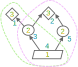
\includegraphics[width=0.30\textwidth]{Bilder/problem_illustration.pdf}
	\vspace{-10pt}
	% Das folgende ist ein Trick, um "Abbilgung x.y" in eine
	% eigene Zeile zu packen. Der Text zwischen [ und ] steht
	% im Abbildungsverzeichnis. Der Text darunter wird
	% tatsächlich angezeigt.
	\caption[Minimalbeispiel zur Teilgraph-Überspringungs-Problematik. Legende wie in \autoref{fig:trans_closures}.]{\unskip}
	Minimalbeispiel zur Teilgraph-Überspringungsproblematik. Legende wie in Abb. \ref{fig:trans_closures}.
	\label{fig:prob_illu}
\end{wrapfigure}

Leider lassen sich bei dem Vergleich zweier Submodelle gemeinsame Teilgraphen nicht gänzlich einsparen, indem der Similarity-Wert über Forks hinaus propagiert wird, um so jedem Knoten im Graph die Summe aller Knotenwerte unter ihm zuzuordnen, da ein gemeinsamer Teilgraph über mehrere Forks betreten werden kann (z.B. der Teilgraph der Schnittmenge von grün und lila in \autoref{fig:trans_closures} kann über Knoten 6 und 5 betreten werden) und nur der maximale Teilgraph gezählt werden darf - ansonsten würde es zu einer doppelten Wertung eines oder mehrerer Knoten kommen. Auch ist die Maximalität  des gemeinsamen Teilgraphen nur mit erheblichen Rechenaufwand, der dem Prinzip des Auslassens entgegensteht, zu überprüfen. Der Graph aus \autoref{fig:prob_illu} ist zur Veranschaulichung geeignet: Es ist schwierig Knoten 4 mit Wert 1 genau einmal zu zählen. Wird Knoten 3 betreten und der restliche Teilgraph (Knoten 4) übersprungen, so wird der Wert 3 zur Similarity addiert.

\chapter{Implementierung} 

Zunächst wird eine Basisimplementation gegeben, die den Algorithmus zur Subproblemerzeugung und Similarity-Berechnung aus \autoref{sec:alg_comp} umsetzt und diesen dann auf Geschwindigkeit optimiert.

\section{Basisimplementation}

\begin{algorithm}
	\caption{Vereinfachter Algorithmus zum Erstellen der Subprobleme aus den Submodellen}\label{lst:create_sub}
	\begin{algorithmic}[1]
		\Procedure{Create Subproblems}{$F$} 
			\For{$S \in atomicSubmodels$}
				\State $S.graph \gets calculateGraph(S)$
				\State $S.graph \gets reduceGraph(S.graph, F)$
			\EndFor \Comment{$n := |atomicSubmodels|$}
			\While{$|atomicSubmodels| \neq 0$} \Comment{$O(\frac{n(n+1)}{2}) \cdot O(t_{sim}) = O(n^2 \cdot t_{sim})$}
				\State $M \gets selectOne(atomicSubmodels)$
				\State $M.set \gets \emptyset$
				\While{$complexity(M) < minSubproblemComplexity$}
					\State $highestSim \gets -1$					
					\For{$S \in atomicSubmodels$}
						\State $sim \gets computeSim(M, S)$
						\If{$sim > highestSim$}
							\State $mostSimilar \gets S$
							\State $highestSim \gets sim$
						\EndIf
					\EndFor
					\State $M \gets M \cup mostSimilar$
					\State $M.set \gets M.set \cup mostSimilar.set$
					\State $atomicSubmodels \gets atomicSubmodels \setminus mostSimilar$
				\EndWhile
				\State $subproblems \gets subproblems \cup \{M\}$
			\EndWhile		
		\EndProcedure
	\end{algorithmic}
\end{algorithm}


\chapter{Ergebnisse} \label{sec:results}

\section{Benötigte Trainingszeit}

\begin{itemize}
    \item Eine Epoche des Pre-Trainings auf dem Combined-Straßendatensatz dauert zwischen 40 und 50 Minuten. 
    \item Eine Epoche des Trainings auf dem BikeSat-Datensatz dauert zwischen 10 und 17 Minuten. 
    \item Die Netze konvergieren nach circa 33-57 Epochen auf beiden Datensätzen. 
    \item Das Training wird immer vorzeitig vor dem Ablaufen der 100 Epochen beendet.
    \item Der zeitliche Mehraufwand durch die Daten-Augmentierung während des Trainings (vgl. \autoref{sec:pre-processing}) 
    liegt im Schnitt bei 3 min 30s pro Epoche.  
\end{itemize}

\section{Pre-Training-Ergebnisse zur Straßenerkennung}

\begin{table}[ht]
	\centering
	\begin{tabular}{l|c|c}
		Modell & \ac{IoU} & \ac{BIoU} \\
		\midrule
        BUNet2 & 57,13 & 76,71 \\ 
        BUNet15 & 60,75 & 80,80 \\ 
        VBUNet & \textbf{64,26} & \textbf{85,64} \\ 
        RBUNet & 61,45 & 83,86 \\ 
        DBUNet & 62,56 & 84,46 \\ 
        
	\end{tabular}
	\caption{Ergebnisse des Pre-Trainings der Modelle auf der Testpartition des Combined-Datensatzes in Prozent.}
	\label{tab:results-roads}
\end{table}

\autoref{tab:results-roads} zeigt die Test-Ergebnisse der Modelle nach Training auf dem Combined-Datensatz 
(vgl. \autoref{sec:pre-training-roads}) in Prozent. Pro Spalte ist das höchste Ergebnis hervorgehoben. 
\ac{BUNet2} und \ac{BUNet15} sind von Grund auf trainiert, während \ac{VBUNet}, \ac{RBUNet} und \ac{DBUNet} einen auf 
ImageNet vortrainierten Encoder aufweisen. Die \ac{BIoU} verwendet wie bei der Radwegerkennung und wie in \autoref{sec:eval:biou} 
festgelegt eine Puffergröße von 15 Pixeln. 

\section{Ergebnisse der Radwegerkennung}

\begin{table}[ht]
	\centering
	\begin{tabular}{l|cc|cc}
        & \multicolumn{2}{c|}{BikeSat} & \multicolumn{2}{c}{Karlsruhe} \\
		Modell & \ac{IoU} & \ac{BIoU} & \ac{IoU} & \ac{BIoU} \\
		\midrule
        BUNet2$^*$ & 23,54 & 47,71 & 01,30 & 34,80 \\ 
        BUNet2$^l$ & 24,48 & 51,77 & 02,19 & 12,11 \\ 
        BUNet2$^r$ & 25,35 & 51,27 & 09,36 & 47,57 \\ 
		\midrule

        BUNet15$^*$ & 27,93 & 56,55 & \textbf{21,52} & \textbf{59,25} \\ 
        BUNet15$^l$ & 28,14 & 57,14 & 16,47 & 54,17 \\ 
        BUNet15$^r$ & 28,22 & 57,26 & 10,17 & 53,81 \\ 
		\midrule

        VBUNet$^*$ & 30,45 & 61,48 & 09,69 & 37,84 \\ 
        VBUNet$^l$ & \underline{\textbf{32,24}} & \textbf{62,93} & 12,85 & 54,91 \\ 
        VBUNet$^r$ & \textbf{31,84} & 61,51 & 17,53 & \textbf{61,51} \\ 
		\midrule

        RBUNet$^*$ & 29,11 & 60,53 & 11,74 & 32,80 \\ 
        RBUNet$^l$ & 30,98 & 60,51 & \underline{\textbf{24,67}} & \underline{\textbf{65,27}} \\ 
        RBUNet$^r$ & 31,31 & \underline{\textbf{63,55}} & \textbf{18,21} & 55,53 \\ 
		\midrule

        DBUNet$^*$ & 30,76 & 61,78 & 07,14 & 45,97 \\ 
        DBUNet$^l$ & 31,55 & 62,38 & 17,47 & 55,20 \\ 
        DBUNet$^r$ & \textbf{32,12} & \textbf{62,99} & 14,03 & 51,73 \\ 
        
	\end{tabular}
	\caption{Ergebnisse der Modelle auf der Testpartition des BikeSat-Datensatzes und dem Karlsruhe-Testdatensatz 
    in Prozent.}
	\label{tab:results}
\end{table}

\begin{table}[ht]
	\centering
	\begin{tabular}{l|cc}
		Modell & \ac{IoU} & \ac{BIoU}  \\
		\midrule
        BUNet2$^*$ & 02,78 & 07,31  \\ 
        BUNet2$^l$ & 04,23 & 09,90  \\ 
        BUNet2$^r$ & 01,94 & 04,67  \\ 
		\midrule

        BUNet15$^*$ & 07,85 & 17,12  \\ 
        BUNet15$^l$ & 05,59 & 10,17  \\ 
        BUNet15$^r$ & 04,94 & 10,06  \\ 
		\midrule

        VBUNet$^*$ & \underline{\textbf{23,80}} & \underline{\textbf{50,45}} \\ 
        VBUNet$^l$ & 11,34 & 22,89 \\ 
        VBUNet$^r$ & \textbf{22,93} & 38,69 \\ 
		\midrule

        RBUNet$^*$ & \textbf{20,97} & \textbf{48,42} \\ 
        RBUNet$^l$ & 04,62 & 08,19 \\ 
        RBUNet$^r$ & 11,58 & 20,49 \\ 
		\midrule

        DBUNet$^*$ & 17,52 & \textbf{43,53} \\ 
        DBUNet$^l$ & 09,73 & 25,43 \\ 
        DBUNet$^r$ & 19,77 & 36,33 \\ 
        
	\end{tabular}
	\caption{Ergebnisse der Modelle auf dem Karlsruhe-Testdatensatz, wobei Bilder mit leeren Masken entfernt wurden, 
    in Prozent.}
	\label{tab:results-ka-small}
\end{table}

\autoref{tab:results} zeigt die Test-Ergebnisse der Modelle nach Training (s. \autoref{sec:training} für Details) auf dem BikeSat-Datensatz 
(s. \autoref{sec:bike-data}) in Prozent. Zusätzlich zeigt die Tabelle die Test-Ergebnisse auf allen 196 $512{\times}512$-Ausschnitten 
des Karlsruhe-Datensatz (s. \autoref{sec:karlsruhe}) in Prozent. Der Karlsruhe-Datensatz in dieser Tabelle
enthält Ausschnitte, die keine Radwege enthalten. \\ 
Pro Spalte sind die höchsten drei Ergebnisse hervorgehoben und das höchste unterstrichen.
Die \ac{BIoU} hat eine Puffergröße von 15 Pixeln, wie in \autoref{sec:eval:biou} festgelegt.

\autoref{tab:results-ka-small} zeigt die Test-Ergebnisse der Modelle aus \autoref{tab:results} auf allen 49 $512{\times}512$-Ausschnitten, 
\textit{die Radwegen enthalten}, des Karlsruhe-Datensatz (s. \autoref{sec:karlsruhe}) in Prozent. 
Ein Ausschnitt enthält einen Radweg, wenn in der zugehörigen Label-Maske mindestens ein Pixel als Radweg annotiert ist. \\
Pro Spalte sind die höchsten drei Ergebnisse hervorgehoben und das höchste unterstrichen.
Die \ac{BIoU} hat eine Puffergröße von 15 Pixeln, wie in \autoref{sec:eval:biou} festgelegt.

% networks tested with karlsruhe test data set  

% testing ./../Models/Double-Data\backbones\bike_mapper_pre-train-scratch-densenet121_Aug_IoU3076_q6178.h5
% iou: 0.07135618478059769, quality:0.45967867970466614

% testing ./../Models/Double-Data\backbones\bike_mapper_pre-train-scratch-resnet34_Aug_IoU2911_q6053.h5
% iou: 0.11737822741270065, quality:0.3280484974384308

% testing ./../Models/Double-Data\backbones\bike_mapper_pre-train-scratch-vgg16_Aug_IoU3045_q6148.h5
% iou: 0.09694375097751617, quality:0.3783626854419708

% testing ./../Models/Double-Data\pre-train\bike_mapper_pre-train-freeze-left_Aug_IoU2448_q5177.h5
% iou: 0.020918812602758408, quality:0.1211065948009491

% testing ./../Models/Double-Data\pre-train\bike_mapper_pre-train-freeze-right_Aug_IoU2535_q5127.h5
% iou: 0.09364935010671616, quality:0.47571051120758057

% testing ./../Models/Double-Data\pre-train\bike_mapper_triple-param_pre-train-freeze-left_Aug_IoU2814_q5714.h5
% iou: 0.1647404581308365, quality:0.5417148470878601

% testing ./../Models/Double-Data\pre-train\bike_mapper_triple-param_pre-train-freeze-right_Aug_IoU2822_q5726.h5
% iou: 0.10167630761861801, quality:0.5381019115447998

% testing ./../Models/Double-Data\road-pre-trained-backbones\bike_mapper_pre-train-densenet121freeze-left_Aug_IoU3155_q6238.h5
% iou: 0.17469285428524017, quality:0.5520145893096924

% testing ./../Models/Double-Data\road-pre-trained-backbones\bike_mapper_pre-train-densenet121freeze-right_Aug_IoU3212_q6299.h5
% iou: 0.14031212031841278, quality:0.5172706246376038

% testing ./../Models/Double-Data\road-pre-trained-backbones\bike_mapper_pre-train-resnet34freeze-left_Aug_IoU3098_q6051.h5
% iou: 0.24674279987812042, quality:0.6527144312858582

% testing ./../Models/Double-Data\road-pre-trained-backbones\bike_mapper_pre-train-resnet34freeze-right_Aug_IoU3131_q6355.h5
% iou: 0.18207795917987823, quality:0.5552724599838257

% testing ./../Models/Double-Data\road-pre-trained-backbones\bike_mapper_pre-train-vgg16freeze-left_Aug_IoU3224_q6293.h5
% iou: 0.12852726876735687, quality:0.5490880012512207

% testing ./../Models/Double-Data\road-pre-trained-backbones\bike_mapper_pre-train-vgg16freeze-right_Aug_IoU3184_q6151.h5
% iou: 0.175296351313591, quality:0.6151095628738403

% testing ./../Models/Double-Data\bike_mapper_scratch_Aug_IoU2354_q4771.h5
% iou: 0.013092363253235817, quality:0.3479517698287964

% testing ./../Models/Double-Data\bike_mapper_scratch_triple-param_Aug_IoU2793_q5655.h5
% iou: 0.21523651480674744, quality:0.5924956798553467


\chapter{Diskussion}

Im Folgenden werden die zuvor präsentierten Ergebnisse diskutiert. Zunächst werden die beobachteten Phänomene 
bei der Straßenerkennung betrachtet und daraufhin die bei der Radwegerkennung.

\section{Straßenerkennung}

Die Ergebnisse der Straßenerkennung können als gut im Vergleich zur Literatur eingeordnet werden. 
Das beste Modell ist hierbei das \ac{VBUNet}, welches mit einer Test-IoU von 64,26\% mit den 
performantesten Modellen aus \autoref{sec:state-of-the-art-roads} mithalten kann. Hier wurden 
Spitzenwerte von 67,10 und 65,60\% auf dem Massachusetts- bzw. Deep-Globe-Datensatz erzielt. 
Die Hyperparameter dieser Modelle sind auf das jeweilige Problem optimiert, während das VBUNet nicht optimiert ist. 
Dafür sind die Ergebnisse sehr gut. \\  
Was überraschend ist, ist, dass im Pre-Training in dieser Arbeit 
das VBUNet die besten Ergebnisse erzielt, während in der Literatur die besten Modelle ResNet-Derivate sind. 
Das kann daran liegen, dass in der Literatur die Modelle isoliert auf dem Massachusetts- und Deep-Globe-Datensatz 
trainiert werden. In dieser Arbeit sind alle Netze hingegen auf der Vereinigung der beiden Datensätze trainiert. 
Die beiden Datensätze stellen allerdings sehr unterschiedliche Landschaften dar. 
Möglicherweise funktioniert also ResNet, welches eine viel höhere Komplexität als VGG aufweist, besser 
als Spezialisierung auf einer der beiden Landschaften, ist also besonders angepasst auf die jeweilige Landschaft, 
während VGG mit der geringeren Komplexität besser Straßen generalisieren kann und deshalb robuster ist. 
Eine weitere, simplere Erklärung ist, dass in dieser Arbeit die Netze lediglich mit einem Satz 
an Hyperparametern und einem festen Seed genau ein mal trainiert sind. Außerdem sind die Ergebnisse 
nicht mit einer Kreuzvalidierung überprüft.
Es kann also lediglich eine schlechte Besetzung der Hyperparameter und Startwerte für das ResNet und eine 
gute für VGG vorliegen. \\
Der Erwartung entsprechend kann BUNet2 mit der eher geringen Parameteranzahl von 2 Mio. Parametern nicht 
mit der Leistung der restlichen Netze konkurrieren. BUNet15 zeigt, dass BUNet2 schlicht eine zu geringe 
Komplexität aufweist, um die Straßen so gut wie die komplexeren Netze segmentieren zu können. 
Trotzdem ist die Leistung nicht schlecht. Mit nur einem Bruchteil der Parameter der übrigen Netze
kann BUNet2 zumindest vergleichbare Ergebnisse erzeugen. \\
Während BUNet15 und BUNet2 bis auf die Parameteranzahl identisch sind, weswegen sich ein Unterschied in der 
Performance auf den Komplexitätsunterschied zurückführen lässt, ist bei dem Performance-Unterschied 
zwischen BUNet15 und den Backbone-Architekturen, insbesondere RBUNet und DBUNet, unklar, ob die kleine 
Differenz von wenigen Prozenten in der IoU bzw. der BIoU in der unterschiedlichen Architektur oder dem 
Pre-Training der Backbone-Architekturen auf ImageNet begründet ist. Eventuell ist RBUNet z.B. die schlechtere 
Architektur, erzielt aber bessere Ergebnisse als BUNet15 aufgrund des Pre-Trainings auf ImageNet. 
Ob das der Fall ist, kann nur durch weitere Experimente geklärt werden, die BUNet15 mit den nicht vortrainierten 
Backbone-Netzen vergleicht. In jedem Fall scheint aber das Pre-Training auf ImageNet nur geringe 
Performance-Verbesserungen herbeizuführen. 

\subsection{BIoU für die Straßenerkennung}

\begin{wrapfigure}{r}{0.40\textwidth}
	\centering
	\vspace{-20pt} % Manchmal möchte man den oberen Abstand selbst anpassen
	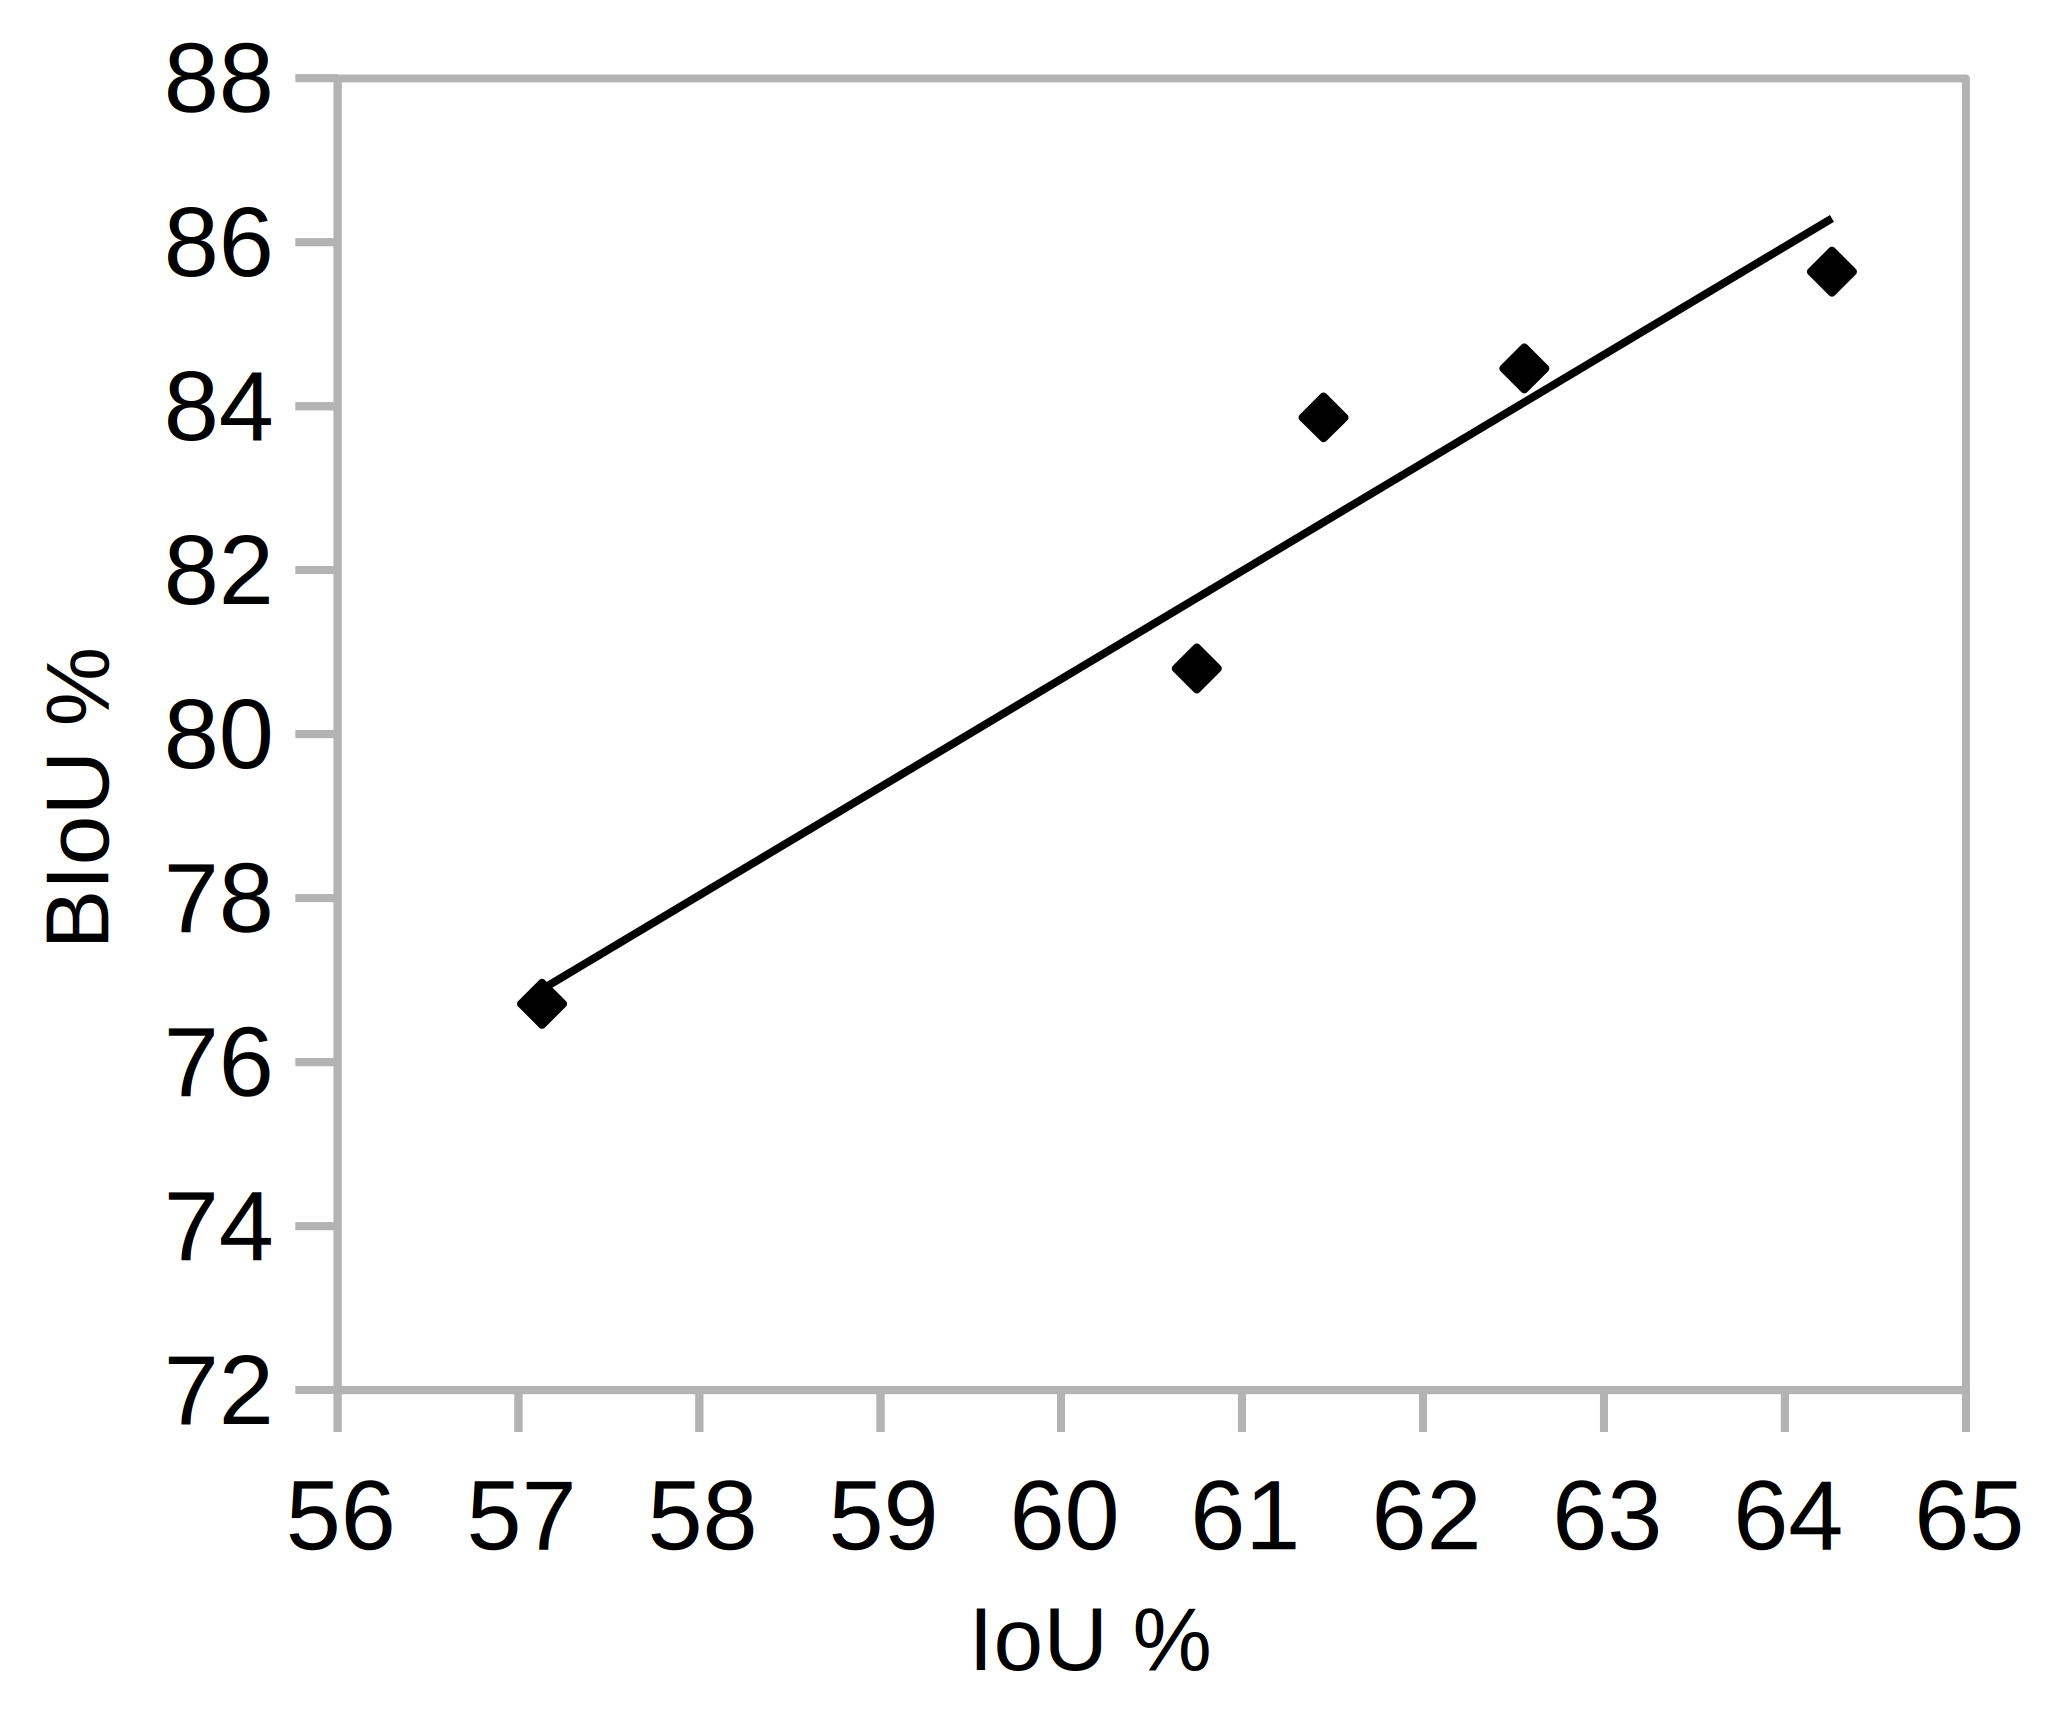
\includegraphics[width=0.35\textwidth]{Bilder/iou-biou-correlation.pdf}
	\vspace{-5pt}
	% Das folgende ist ein Trick, um "Abbilgung x.y" in eine
	% eigene Zeile zu packen. Der Text zwischen [ und ] steht
	% im Abbildungsverzeichnis. Der Text darunter wird
	% tatsächlich angezeigt.
	\caption[BIoU der Modelle der Straßenerkennung aufgetragen über deren IoU.]{\unskip}
	BIoU über IoU in Prozent (Straßenerkennung). Pos. Korrelation mit $r = 0,9707$. 
	\label{fig:iou-biou-corr}
	% \vspace{-20pt}
\end{wrapfigure}

Im Gegensatz zu den Radweg-Datensätzen bei der Maskenerstellung des Straßendatensatzes keinerlei Schätzung 
über die Lage der Wege eingesetzt worden. Die Masken sind also überwiegend deckungsgleich mit den tatsächlichen 
Straßen im Input-Bild, während bei den Radwegen manche Radwege grob versetzt positioniert sind. 
Deswegen muss die BIoU bei der Straßenerkennung keine komplette Verschiebung der Prediction zur Ground-Truth ausgleichen, 
sondern glättet lediglich die IoU im Randbereich der Straßen. Daher ist die Straßenerkennung geeignet, 
um zu untersuchen, ob die BIoU erwartungsgemäß arbeitet. \autoref{fig:iou-biou-corr} zeigt die Testergebnisse der 
Straßenerkennung mit der BIoU in Prozent aufgetragen über der IoU in Prozent für die jeweiligen Modelle. 
Es herrscht eine starke positive Korrelation zwischen der IoU und BIoU mit Korrelationskoeffizient $r = 0,9707$. 
Die starke Korrelation spricht für die vorangegangene Annahme, dass im Falle der Straßendetektion die BIoU 
ungerade Predictions glättet und fairer bewertet, bzw. näher an dem ist, wie ein Mensch die Performanz der 
Netze wahrnimmt. Die sehr streng bewertende IoU gibt einen schlechten Eindruck von der Leistungsfähigkeit des Netzes. 
Aus den Beispielpredictions der Straßenerkennung erhält ein menschlicher Beobachter nicht den Eindruck, 
dass nur circa 60\% der Straßen richtig erkannt worden sind, sondern eher im Bereich von 80\% oder mehr. 
Damit beweist sich die BIoU, als ein Maß, welches im Falle der Straßenerkennung lediglich die IoU so anhebt, 
dass eine zu schmal oder zu breit gezeichnete Predicition mit rauen Kanten als (qualitativ) korrekt in 
die Bewertung einfließt.  

\section{Radwegerkennung} \label{sec:disc:recog}

Die Ergebnisse für die Radwegerkennung (vgl. \autoref{tab:results}) zeigen, dass die Ergebnisse der 
Radwegerkennung statistisch signifikant\footnote{
	$p = 1,887\cdot 10^{-8}$ für IoU und $p = 3,77\cdot 10^{-7}$ für BIoU
	des einseitigen Zweistichproben-Welch-Test zwischen der Straßenerkennung 
	und der Radwegerkennung für Basic-Aug. 
} schlechter sind, als die der Straßenerkennung. Hierfür gibt es folgende Gründe:
\begin{enumerate}
	\item Das Problem der Radwegerkennung ist schwerer. Für die Radwegerkennung fällt es selbst Menschen schwer 
	diese auf Satellitenbildern zu erkennen. Für Fahrradstreifen am Straßenrand ist das noch gut möglich, 
	aber für oft überdeckte und überschattete Fahrradwege neben der Straße, die zum Beispiel durch einen Grünstreifen 
	von der Straße getrennt sind und mit dem Fußweg verbunden sind, ist schwierig festzustellen, ob ein Radweg 
	vorhanden ist, oder ob es sich nur um einen Gehweg handelt. Außerdem weisen Radwege weitaus 
	heterogenere Beläge auf, als städtische Straßen. Für Radwege kommen Asphalt, unterschiedlich farbene Pflastersteine,
	Schotter, rot oder grün gefärbter Asphalt und andere Untergründe zum Einsatz, 
	während die allermeisten Straßen in der Stadt aus Asphalt bestehen.
	Weiterhin gibt es viel weniger Radwege als Straßen, wodurch in den Trainingsdaten eine große Imabalance 
	und generell weniger Beispiele vorhanden sind, als in einem ähnlich großen Datensatz für die Straßenerkennung. 
	Auch unterscheiden sich Radwege zwischen Ländern und selbst Städten eines Landes weitaus stärker, als Straßen.
	\item Die automatisch generierten Annotationen sind überwiegend (ca. zu 83\%; vgl. \autoref{sec:quality-of-masks})
	auf dem Niveau einer Annotation durch Menschen, allerdings könnte der Anteil der Annotationen, die schlichtweg
	falsch sind, die Ergebnisse stark beeinträchtigen. Um diese Hypothese zu verifizieren sind weitere 
	Experimente mit einem besser annotierten Datensatz notwendig. Ein durch Menschen annotierter Datensatz 
	muss dafür klar definieren, was die Labelnden als Radweg anerkennen, da bei Radwegen auf Luftbildern 
	nicht unbedingt ein allgemeiner Konsens besteht, was als Radweg zu markieren zählt. Durch menschliche Annotation 
	kann aber zumindest ausgeschlossen werden, dass Pixel als Radweg annotiert sind, die eine Wiese oder ein Gebäude zeigen.
	\item Möglicherweise ist die semantische Segmentierung zum Erkennen der Radwege eine zu detaillierte Methode. 
	Um die Forschungsfrage dieser Arbeit -- existiert ein Radweg an dieser Straße und wenn ja, in welche Richtung -- 
	zu beantworten, ist die semantische Segmentierung der Radwege übermäßig. Die semantische Segmentierung 
	schafft mehr Informationen, als benötigt werden. Das bietet zwar auch Vorteile, dass zum Beispiel der Radweg 
	auf einem Luftbild als solcher eingefärbt werden kann, aber verlangt auch weitaus genauere Annotationen. \\
	Eine Alternative Herangehensweise kann sein, das Problem so zu modellieren, dass die Modelle direkt einen Graphen
	an Radwegen extrahieren, anstatt zuerst die zum Radweg gehörigen Pixel zu annotieren und die Graphenextraktion 
	in einem externen Schritt vorzunehmen. Dabei können als Label direkt die Graphen aus \ac{OSM} verwendet werden 
	und die Rad\textit{streifen} müssen nicht verschoben werden. Das Problem hierbei ist, zu Kodieren, ob 
	ein Radweg rechtsseitig oder linksseitig vorliegt, da die Definition von rechts- und linksseitig abhängt  
	von dem von \ac{OSM} willkürlich gewählten Verlauf der Straße. Hierfür könnte der Begriff von links- und 
	rechtsseitig transformiert werden in östlich und nördlich, bzw. in westlich und südlich von der Straße.    
\end{enumerate}
Obwohl die Radwegerkennung nicht so gute Ergebnisse liefert, wie die Straßenerkennung, und die Ergebnisse 
für die Radwegerkennung durchaus Verbesserungspotential bieten, lässt sich aus der Arbeit 
schließen, dass es möglich ist, andere Strukturen der städtischen Infrastruktur aus Luftbildern zu erkennen, 
als Straßen. 

\subsection{Ergebnisse auf Karlsruhe gegenüber BikeSat und Wolfsburg}

Aus allen Experimenten geht hervor, dass die Performance auf dem (ungefilterten und gefilterten) Karlsruhe-Datensatz deutlich schlechter ist, 
als auf dem BikeSat- und Wolfsburg-Datensatz. Außerdem hat die Color-Aug. keine Verbesserung gegenüber 
Basic-Aug. hervorgerufen. Auch ist der Wolfsburg-Datensatz, der eine andere Stadt, bei gleicher Optik der Bilder, 
zeigt, als der BikeSat-Datensatz, gleich auf mit dem BikeSat-Datensatz. Wolfsburg weist aber eine sehr ähnliche 
Infrastruktur zu den anderen Städten aus Niedersachsen (BikeSat) auf. Daraus lässt sich schließen, 
dass für die schlechte Performance auf dem Karlsruhe-Datensatz wahrscheinlich nicht die Optik der Bilder verantwortlich 
ist, sondern die sehr unterschiedliche Infrastruktur der Fahrradwege oder das allgemeine Stadtbild. 
So hat Karlsruhe beispielsweise deutlich mehr Fahrradstreifen am Straßenrand als die niedersächsischen Städte. 
Diese Beobachtung beantwortet die Forschungsfrage, ob Ergebnisse auf Städten unterschiedlicher Infrastrukturen 
übertragbar sind. So ist eine Übertragung bedingt möglich, aber es liegt nahe, dass mit Performance-Einbußen zu rechnen ist, 
die die Stärke des Unterschieds der Infrastrukturen widerspiegeln. 
Um diese These zu belegen, bedarf es jedoch weiterer Experimente mit mehr Städten. Eventuell ist dann 
auch eine Proportionalität zwischen Performance-Einbußen auf für das Modell unbekannten Städten und der Stärke 
des Unterschieds der Städte erkennbar. Insofern eine Quantifizierung des Unterschieds der Städte gelingt. 

Die signifikant bessere BIoU von Wolfsburg im Gegensatz zu BikeSat wird darauf zurückgeführt, dass 
Wolfsburg eine sehr ähnliche Fahrrad-Infrastruktur aufweist, wie der BikeSat-Datensatz, aber weniger 
Samples beinhaltet, die schwierig als Radweg zu erkennen sind. Außerdem ist der Unterschied nur gering, 
da der Unterschied in IoU keine statistische Signifikanz erreicht. 

% schlechtere Ergebnisse als Straßenkennung, was probleme ? 
% warum karslrueh so viel schlechterbiou
% warum wolfsburg besser ? 
% Wolfsburg doch eher ungeeignet weil zu ähnlich 
% experimente mit anderen städten
% color augmentation nicht viel grebracht -> liegt wohl an stadtbild
% netze eher konservativ wie karlsrueh prediction zeigt
% warum gefilterter schlechter?
% effizienz des pretraining 
% warum wenig unterschiede zwischen den netzen

\subsection{Effektivität des Pre-Trainings}

In dieser Arbeit wird zweimal Pre-Training angewandt: Zunächst sind die Backbone-Netze (VBUNet, RBUNet, DBUNet) 
auf dem ImageNet-Datensatz vortrainiert, während das die BUNet-Netze nicht sind. Dann sind die Netze 
mit \{B,VB,RB,DB\}UNet$^{\{l,r\}}$ auf dem Combined-Datensatz der Straßenerkennung fine-tuned bzw. für die 
Radwegerkennung vortrainiert. Zunächst lässt sich sagen, dass das links- bzw. rechtsseitige Fine-Tuning 
keinen generellen Effekt hat und eher ein Hyperparameter darstellt, welcher pro Modell optimiert werden muss. 
Allgemein erzielt das Pre-Training auf dem Straßendatensatz nur für Basic-Aug. einen positiven Effekt, 
während es für Color-Aug. unterschiedliche Effekte, von destruktiv bis konstruktiv, hat. 
Das scheint zu zeigen, dass durch das Pre-Training im Basic-Aug.-Fall vermutlich die Farbe von Straßen als 
grau (Asphalt) gelernt wird, was bei der Radwegerkennung ohne farbverändernde Augmentierungen hilfreich ist.  
Möglicherweise ist dann die Performance von vortrainierten Modellen mit Color-Aug. schlechter, 
da der Datensatz zu klein ist, um die Struktur anstelle der Farbe ausreichend zu gut zu lernen. \\ 
Bezüglich des Vortrainings auf dem ImageNet-Datensatz lässt sich nicht folgern, 
ob diese Vortrainings-Methode effektiv ist, da es ohne ein Vortraining der BUNet-Modelle auf dem ImageNet-Datensatz 
nicht möglich ist festzustellen, ob die bessere Performance der Backbone-Modelle an dem Pre-Training oder 
besserer Archtiektur liegt. In weiteren Experimenten kann BUNet2 und BUNet15 auf ImageNet vortrainiert werden, 
für eine vergleichbare Gegenüberstellung mit den Backbone-Netzen. \\
Insgesamt spielt das Pre-Training aber eine eher geringe Rolle und kann eher zur Optimierung genutzt werden. 
Davor sollte aber der Datensatz oder die grundlegende Funktionsweise der Radwegerkennung verbessert werden (vgl. \autoref{sec:disc:recog}). 

\subsection{Gefilterter Straßendatensatz}

\newcommand{\overbar}[1]{\mkern 8mu\overline{\mkern-8mu#1\mkern-8mu}\mkern 8mu}

Sei $K_{fil} \subset K_{unfil}$ mit $|K_{fil}| = 49; ~|K_{unfil}| = 196$ der gefilterte Kalrsruhe-Datensatz 
als Teilmenge vom ungefilterten Karlsruhe-Datensatz $K_{unfil}$. Wobei gefiltert bedeutet, dass 
keine leere Ground-Truth-Maske existiert, alle Bilder also einen Radweg enthalten.
Die Ergebnisse aus \autoref{tab:results} und \autoref{tab:results-ka-small} mit der Visualisierung aus 
\autoref{fig:iou-biou-corr-ka} zeigen, dass die BIoU auf dem gefilterten Datensatz $K_{fil}$ signifikant 
schlechter ist, als auf dem ungefilterten. Da die BIoU als aritmethisches Mittel der BIoU-Werte der einzelnen Bilder 
berechnet wird und die Predictions auf den Bildern von $K_{fil} \cap K_{unfil} = K_{fil}$ gleich ausfallen, 
lässt sich aus den durchschnittlichen Ergebnissen den beiden Datensätze die durchschnittliche BIoU auf den leeren Bildern 
$K_{leer} := K_{unfil} \setminus K_{fil};~ |K_{leer}| = |K_{unfil}| - |K_{fil}| = 147$ über   
\begin{align}
	\overbar{BIoU_{K_{unfil}}} = \frac{|K_{fil}| \cdot \overbar{BIoU_{K_{fil}}} + |K_{leer}| \cdot \overbar{BIoU_{K_{leer}}}}{|K_{unfil}|} \nonumber \\
	\label{eq:ka-empty}  \implies \overbar{BIoU_{K_{leer}}} = \frac{|K_{unfil}| \cdot \overbar{BIoU_{K_{unfil}}} - |K_{fil}| \cdot \overbar{BIoU_{K_{fil}}}}{|K_{leer}|} \\ 
	= \frac{196 \cdot \overbar{BIoU_{K_{unfil}}} - 49 \cdot \overbar{BIoU_{K_{fil}}}}{147} \nonumber
\end{align}
berechnen. Das ergibt \\ 
$\overbar{BIoU_{K_{leer}, basic}} = 56,36\%$ und \\ 
$\overbar{BIoU_{K_{leer}, color}} = 45,19\%$
für Basic-Aug. bzw. Color-Aug. Verglichen mit \\ 
$\overbar{BIoU_{K_{fil}, basic}} = 48,16\%; ~\overbar{BIoU_{K_{unfil}, basic}} = 23,58\%$ und \\
$\overbar{BIoU_{K_{fil}, color}} = 42,68\%; ~\overbar{BIoU_{K_{unfil}, color}} = 35,14\%$
sind die Werte also höher. Weiterhin gilt $\forall (x, y) \in K_{leer}: BIoU(Prediction_m(x), y) \in \{0; 1\}$ für alle Modelle $m$. 
Das liegt daran, dass die Ground-Truth $y$ per Definition von $K_{leer}$ stets leer ist, woraus folgt, dass die Kardinalität der 
Schnittmenge mit der Prediction für einen Input $x$ immer $0$ ist. Das heißt, die BIoU ist immer $0$, es sei denn 
das Modell $m$ annotiert keine Pixel als Radwege, dann ist die Kardinalität der Vereinigungsmenge auch $0$ und 
die BIoU per Definition gleich $1$. Selbige Schlussfolgerung gilt analog für die IoU. \\ 
Aus den Werten für $BIoU_{K_{leer}}$ folgt, dass in circa der Hälfte der Fälle die Modelle keinen einzigen Pixel 
(fälschlicherweise) als Radweg annotieren. Zusammen mit den Beispiel-Predictions aus \autoref{sec:example-preds} 
liegt die Vermutung sehr nahe, dass in der anderen Hälfte der Fälle nur sehr wenige Pixel von den Modellen 
fälschlicherweise als Radweg erkannt wurden. Daraus lässt sich eine sehr gute True-Negative-Rate und 
geringe False-Positive-Rate schließen, 
für deren Bewertung die ausgewählten Maßzahlen IoU und BIoU äußerst ungeeignet sind. Insofern lässt sich 
also ein gutes Ergebnis verzeichnen, dass die Modelle nicht jegliche Straßen mit Radwegen versehen und 
korrekt gelernt haben, was keine Radwege sind, obwohl die Modelle während des Trainings mit dem BikeSat-Datensatz 
nur Beispiele eingegeben bekommen haben, die Radwege enthalten. Es folgt, dass die Modelle eher hesitent sind,
Pixel als Radwege zu annotieren.  

% \subsection{BIoU für Radwegerkennung}

\chapter{Fazit}

Abschließend lässt sich zusammenfassen, dass die Radwegerkennung auf dem BikeSat und Wolfsburg-Datensatz 
ausreichend gut funktioniert hat, aber auf Städten anderer Infrastruktur, wie Karlsruhe, eher mangelhaft.
Die Übertragbarkeit von Ergebnissen zwischen unterschiedlichen Städten und Ländern ist daher, zumindest 
für den Fall der Radwegerkennung, eher schwierig. Mit dem BikeSat-, Wolfsburg- und Karlsruhe-Datensatz 
sind allerdings Datensätze geschaffen, die weiter für die Radwegerkennung aus Luftbildern verwendet 
werden können, um z.B. andere Herangehensweisen zu untersuchen. Die Datensätze sind dabei vom Umfang 
vergleichbar mit Benchmark-Datensätzen der Straßenerkennung. \\
Außerdem zeigt die Arbeit, dass Erkennung von feineren Strukturen der Infrastruktur von Städten als Straßen 
möglich ist. Für die bessere und intuitivere Einordnung von Ergebnissen der semantischen Segmentierung, 
bei denen die exakte Position weniger relevant ist, zeigt sich die in dieser Arbeit aus der Quality entwickelte \ac{BIoU} 
als nützliches Werkzeug und Bewertungsmaß, welches im praktischen Einsatz die Erwartungen erfüllt. \\
Das überwachte Pre-Training auf Straßendatensätzen und unterschiedliche Modellarchitekturen 
erzeugen keine signifikanten Unterschiede in der Performance. 

Als Zukunftsausblick können auf Basis dieser Arbeit andere Infrastruktur-Elemente in Städten erkannt werden, 
wie Busspuren, Gehwege, Parkplätze am Straßenrand oder sonstiges. 
Möglicherweise kann mit dem direkten Extrahieren der Graphen von z.B. Radwegen einige Probleme mit dem automatischen 
Annotieren der Datensätze umgangen werden und somit bessere Ergebnisse erzielt werden. 
Auch könnte ein unüberwachtes Pre-Training auf einem sehr großen Datensatz mit sehr vielen unterschiedlichen 
Städten einen Vorteil bringen. Außerdem kann untersucht werden, wie viel Einfluss die unterschiedliche 
Infrastruktur hat, und inwiefern diese die Ergebnisse verschlechtert. 
Des Weiteren sollte beachtet werden, dass die Datensätze zur Radwegerkennung in dieser Arbeit 
eine \ac{GSD} von 20 $\frac{cm}{Pixel}$ aufweisen, weswegen auf Zoom-Augmentierung verzichtet wird. 
Sollten unterschiedliche \acp{GSD} in zukünftigen Arbeiten verwendet werden, sollte diese Augmentierung 
untersucht werden. 


% ---- Literaturverzeichnis
\cleardoublepage
\renewcommand*{\chapterpagestyle}{plain}
\pagestyle{plain}
\pagenumbering{Roman}                   % Römische Seitenzahlen
\setcounter{page}{\numexpr\value{savepage}+1}
\printbibliography[title=Literaturverzeichnis]

% ---- Anhang
\appendix
\chapter{Anhang}

\section{Architekturen}

\begin{figure}
	\centering
	\includegraphics[width=0.8\textwidth]{Bilder/vgg16-architecture.pdf} 
	\caption{Die ursprünglichen VGG-Architekturen. Spalte D zeigt VGG16 wie in \autoref{sec:pretrained-backbones:vgg16} beschrieben. Abb. aus \cite{Simonyan.04092014}.}
	\label{fig:vgg16-architecture}
\end{figure} 

\begin{figure}
	\centering
	\includegraphics[width=0.8\textwidth]{Bilder/resnet34-architecture.pdf} 
	\caption{Die ursprünglichen ResNet-Architekturen. Zwischen jeweils zwei Convolutional-Layer befindet sich eine Skip-Connection \cite{He.10122015}.}
	\label{fig:resnet34-architecture}
\end{figure} 

\begin{figure}
	\centering
	\includegraphics[width=0.8\textwidth]{Bilder/densenet121-architecture.pdf} 
	\caption{Die ursprünglichen DenseNet-Architekturen \cite{Huang.25082016}.}
	\label{fig:densenet121-architecture}
\end{figure} 

\pagebreak

\section{Quelltext-Implementation}

\lstinputlisting[
	label=code:quality,    % Label; genutzt für Referenzen auf dieses Code-Beispiel
	caption=Implementation des Quality-Maßes in Python zur Verwendung im Training und Testen von Keras-Modellen.,
	captionpos=b,               % Position, an der die Caption angezeigt wird t(op) oder b(ottom)
	style=EigenerPythonStyle,   % Eigener Style der vor dem Dokument festgelegt wurde
	firstline=1,                % Zeilennummer im Dokument welche als erste angezeigt wird
	lastline=50                 % Letzte Zeile welche ins LaTeX Dokument übernommen wird
]{Quellcode/quality.py}

\pagebreak 

\section{Beispiel-Predictions Karlsruhe}

\begin{figure}
	\centering
	\includegraphics[width=.41\textwidth]{Bilder/Samples-KA/bunet2-l.png} 
	\caption{Beispiel-Predictions des $BUNet2^l$ auf dem Karlsruhe-Datensatz.}
	\label{fig:ka-samples-bunet2-l}
\end{figure}

\begin{figure}
	\centering
	\includegraphics[width=.41\textwidth]{Bilder/Samples-KA/bunet2-r.png} 
	\caption{Beispiel-Predictions des $BUNet2^r$ auf dem Karlsruhe-Datensatz.}
	\label{fig:ka-samples-bunet2-r}
\end{figure}

\begin{figure}
	\centering
	\includegraphics[width=.41\textwidth]{Bilder/Samples-KA/bunet2-s.png} 
	\caption{Beispiel-Predictions des $BUNet2^*$ auf dem Karlsruhe-Datensatz.}
	\label{fig:ka-samples-bunet2-s}
\end{figure}

\begin{figure}
	\centering
	\includegraphics[width=.41\textwidth]{Bilder/Samples-KA/bunet15-l.png} 
	\caption{Beispiel-Predictions des $BUNet15^l$ auf dem Karlsruhe-Datensatz.}
	\label{fig:ka-samples-bunet15-l}
\end{figure}

\begin{figure}
	\centering
	\includegraphics[width=.41\textwidth]{Bilder/Samples-KA/bunet15-r.png} 
	\caption{Beispiel-Predictions des $BUNet15^r$ auf dem Karlsruhe-Datensatz.}
	\label{fig:ka-samples-bunet15-r}
\end{figure}

\begin{figure}
	\centering
	\includegraphics[width=.41\textwidth]{Bilder/Samples-KA/bunet15-s.png} 
	\caption{Beispiel-Predictions des $BUNet15^*$ auf dem Karlsruhe-Datensatz.}
	\label{fig:ka-samples-bunet15-s}
\end{figure}

\begin{figure}
	\centering
	\includegraphics[width=.41\textwidth]{Bilder/Samples-KA/dbunet-l.png} 
	\caption{Beispiel-Predictions des $DBUNet^l$ auf dem Karlsruhe-Datensatz.}
	\label{fig:ka-samples-dbunet-l}
\end{figure}

\begin{figure}
	\centering
	\includegraphics[width=.41\textwidth]{Bilder/Samples-KA/dbunet-r.png} 
	\caption{Beispiel-Predictions des $DBUNet^r$ auf dem Karlsruhe-Datensatz.}
	\label{fig:ka-samples-dbunet-r}
\end{figure}

\begin{figure}
	\centering
	\includegraphics[width=.41\textwidth]{Bilder/Samples-KA/dbunet-s.png} 
	\caption{Beispiel-Predictions des $DBUNet^*$ auf dem Karlsruhe-Datensatz.}
	\label{fig:ka-samples-dbunet-s}
\end{figure}

\begin{figure}
	\centering
	\includegraphics[width=.41\textwidth]{Bilder/Samples-KA/rbunet-l.png} 
	\caption{Beispiel-Predictions des $RBUNet^l$ auf dem Karlsruhe-Datensatz.}
	\label{fig:ka-samples-rbunet-l}
\end{figure}

\begin{figure}
	\centering
	\includegraphics[width=.41\textwidth]{Bilder/Samples-KA/rbunet-r.png} 
	\caption{Beispiel-Predictions des $RBUNet^r$ auf dem Karlsruhe-Datensatz.}
	\label{fig:ka-samples-rbunet-r}
\end{figure}

\begin{figure}
	\centering
	\includegraphics[width=.41\textwidth]{Bilder/Samples-KA/rbunet-s.png} 
	\caption{Beispiel-Predictions des $RBUNet^*$ auf dem Karlsruhe-Datensatz.}
	\label{fig:ka-samples-rbunet-s}
\end{figure}

\begin{figure}
	\centering
	\includegraphics[width=.41\textwidth]{Bilder/Samples-KA/vbunet-l.png} 
	\caption{Beispiel-Predictions des $VBUNet^l$ auf dem Karlsruhe-Datensatz.}
	\label{fig:ka-samples-vbunet-l}
\end{figure}

\begin{figure}
	\centering
	\includegraphics[width=.41\textwidth]{Bilder/Samples-KA/vbunet-r.png} 
	\caption{Beispiel-Predictions des $VBUNet^r$ auf dem Karlsruhe-Datensatz.}
	\label{fig:ka-samples-vbunet-r}
\end{figure}

\begin{figure}
	\centering
	\includegraphics[width=.41\textwidth]{Bilder/Samples-KA/vbunet-s.png} 
	\caption{Beispiel-Predictions des $VBUNet^*$ auf dem Karlsruhe-Datensatz.}
	\label{fig:ka-samples-vbunet-s}
\end{figure}
%\clearpage
%\pagenumbering{Roman}  % römische Seitenzahlen für Anhang

\newpage
\end{document}
